% !TEX TS-program = XeLaTeX
% !TEX encoding = UTF-8 Unicode

%%%%%%%%%%%%%%%%%%%%%%%%%%%%%%%%%%%%%%%%%%%%%%%%%%%%%%%%%%%%%%%%%%%%%%
%
%  哈尔滨工程大学本硕博论文 XeLaTeX 模版 —— 主文件 main.tex
%
%  版本:1.0.0
%  最后更新:
%  修改者:Leo LiWenhui lwh@hrbeu.edu.cn
%  修订者:
%  编译环境1:Ubuntu 12.04 + TeXLive 2013/2014
%  编译环境2:Windows 7/8  + TeXLive 2013/2014
%
%%%%%%%%%%%%%%%%%%%%%%%%%%%%%%%%%%%%%%%%%%%%%%%%%%%%%%%%%%%%%%%%%%%%%%

%%----------  以下是学位、学科类型与打印方式选择 ---------------------

%%----  1.选择学位论文类型,可以是:
%%   Doctor    -博士
%%   Master    -硕士
%%   Bachelor  -学士
\def\xuewei{Doctor}

%%  2.定义学科,可以是:
%%  Engineering   -工学
%%  Science       -科学
%%  Management    -管理
%%  Arts          -艺术
%%  Philosophy    -哲学
%%  Economics     -经济
%%  Laws          -法律
%%  Education     -教育
%%  History       -历史
\def\xueke{Engineering}

%%  3.选择字体,可以是:
%%   adobefont     -Adobe 汉字库
%%   windowsfont   -Windows系统汉字库
%%   linuxfont     -Linux 系统字库
\def\fontselect{adobefont}

%%  4.选择打印单双面打印方式,可以是:
%%   oneside     -单面打印
%%   twoside     -双面打印
\def\oneortwoside{twoside}


%%----------  论文基本格式设置  -------------------------------------

\documentclass[12pt, a4paper, openany, \oneortwoside]{book}

% 字体配置文件
% !TEX TS-program = XeLaTeX
% !TEX encoding = UTF-8 Unicode

%%%%%%%%%%%%%%%%%%%%%%%%%%%%%%%%%%%%%%%%%%%%%%%%%%%%%%%%%%%%%%%%%%%%%%
%
%  哈尔滨工程大学学位论文 XeLaTeX 模版 —— 字体配置文件 fonts.tex
%
%  版本:1.0.0
%  最后更新:
%  修改者:Leo LiWenhui lwh@hrbeu.edu.cn
%  修订者:
%  编译环境1:Ubuntu 12.04 + TeXLive 2013/2014
%  编译环境2:Windows 7/8  + TeXLive 2013/2014
%
%%%%%%%%%%%%%%%%%%%%%%%%%%%%%%%%%%%%%%%%%%%%%%%%%%%%%%%%%%%%%%%%%%%%%%

\usepackage{fontspec}
\usepackage{xltxtra,xunicode}
\usepackage[CJKnumber,CJKchecksingle,slantfont,boldfont]{xeCJK} % 允许斜体和粗体
\usepackage{amsmath}
\usepackage{amssymb}
\usepackage{bm}

\newif\iffontselectadobefont
\newif\iffontselectwindowsfont
\newif\iffontselectlinuxfont

\def\temp{adobefont}
\ifx\temp\fontselect
  \fontselectadobefonttrue  \fontselectwindowsfontfalse  \fontselectlinuxfontfalse
\fi

\def\temp{windowsfont}
\ifx\temp\fontselect
  \fontselectadobefontfalse  \fontselectwindowsfonttrue  \fontselectlinuxfontfalse
\fi

\def\temp{linuxfont}
\ifx\temp\fontselect
  \fontselectadobefontfalse  \fontselectwindowsfontfalse  \fontselectlinuxfonttrue
\fi

\iffontselectadobefont
    % 字体设置特别推荐方案,需要安装 Adobe字体
    % 英文字体设置
    \setmainfont[Mapping=tex-text]{Times New Roman} %衬线字体
    \setsansfont[Mapping=tex-text]{Arial}           %无衬线字体
    \setmonofont[Mapping=tex-text]{Consolas}        %等宽字体

    % 中文字体设置,使用的是 Adobe 字体,保证了在 Adobe Reader / Acrobat 下优秀的显示效果
    \setCJKmainfont[BoldFont={Adobe Heiti Std}, ItalicFont={Adobe Kaiti Std}]{Adobe Song Std}
    \setCJKsansfont{Adobe Heiti Std}
    \setCJKmonofont{Adobe Fangsong Std}

    % 定义字体名称,可在此添加自定义的字体
    \setCJKfamilyfont{song}{Adobe Song Std}
    \setCJKfamilyfont{hei}{Adobe Heiti Std}
    \setCJKfamilyfont{kai}{Adobe Kaiti Std}
    \setCJKfamilyfont{fs}{Adobe Fangsong Std}
    %\setCJKfamilyfont{xkai}{STXingkai}
\fi

\iffontselectwindowsfont
    % 英文字体设置
    \setmainfont[Mapping=tex-text]{Times New Roman} %衬线字体
    \setsansfont[Mapping=tex-text]{Arial}           %无衬线字体
    \setmonofont[Mapping=tex-text]{Courier New}     %等宽字体

    % 中文字体设置,使用的是 Windows 系统字体
	\setCJKmainfont[BoldFont={SimHei}, ItalicFont={KaiTi}]{NSimSun}
	\setCJKsansfont{SimHei}
	\setCJKmonofont{FangSong}

	\setCJKfamilyfont{song}{NSimSun}
	\setCJKfamilyfont{hei}{SimHei}
	\setCJKfamilyfont{kai}{KaiTi}   % XP对应 KaiTi_GB2312,Vista对应KaiTi,注意根据系统切换
	\setCJKfamilyfont{fs}{FangSong} % XP对应 FangSong_GB2312,Vista对应FangSong,注意根据系统切换
\fi

\iffontselectlinuxfont
    % 经典 Linux 英文字体设置方案
    \setmainfont[Mapping=tex-text]{LMRoman10} %衬线字体
    \setsansfont[Mapping=tex-text]{LMSans10}  %无衬线字体
    \setmonofont[Mapping=tex-text]{LMMono10}  %等宽字体

    % 中文字体设置,使用的是 Adobe 字体,保证了在 Adobe Reader / Acrobat 下优秀的显示效果
    \setCJKmainfont[BoldFont={Adobe Heiti Std}, ItalicFont={Adobe Kaiti Std}]{Adobe Song Std}
    \setCJKsansfont{Adobe Heiti Std}
    \setCJKmonofont{Adobe Fangsong Std}

    % 定义字体名称,可在此添加自定义的字体
    \setCJKfamilyfont{song}{Adobe Song Std}
    \setCJKfamilyfont{hei}{Adobe Heiti Std}
    \setCJKfamilyfont{kai}{Adobe Kaiti Std}
    \setCJKfamilyfont{fs}{Adobe Fangsong Std}
    %\setCJKfamilyfont{xkai}{STXingkai}
\fi

\newcommand{\song}{\CJKfamily{song}}
\newcommand{\hei}{\CJKfamily{hei}}
\newcommand{\kai}{\CJKfamily{kai}}
\newcommand{\fs}{\CJKfamily{fs}}

% 定义CJK兼容的汉字字体别名
\def\songti{\song}
\def\fangsong{\fs}
\def\kaishu{\kai}
\def\heiti{\hei}

% 字号
\newcommand{\chuhao}{\fontsize{42pt}{50.5pt}\selectfont}    % 初号,1.25  倍行距
\newcommand{\xiaochu}{\fontsize{36pt}{45pt}\selectfont}     % 小初,1.25  倍行距
\newcommand{\yihao}{\fontsize{26pt}{39pt}\selectfont}       % 一号,1.5  倍行距
\newcommand{\xiaoyi}{\fontsize{24pt}{30pt}\selectfont}      % 小一,1.25 倍行距
\newcommand{\erhao}{\fontsize{22pt}{27.5pt}\selectfont}     % 二号,1.25 倍行距
\newcommand{\xiaoer}{\fontsize{18pt}{22.5pt}\selectfont}    % 小二,1.25 倍行距
\newcommand{\sanhao}{\fontsize{16pt}{20pt}\selectfont}      % 三号,1.25 倍行距
\newcommand{\xiaosan}{\fontsize{15pt}{19pt}\selectfont}     % 小三,1.25 倍行距
\newcommand{\sihao}{\fontsize{14pt}{17.5pt}\selectfont}     % 四号,1.25倍行距
\newcommand{\daxiaosi}{\fontsize{12pt}{18pt}\selectfont}    % 小四,1.5 倍行距
\newcommand{\xiaosi}{\fontsize{12pt}{15pt}\selectfont}      % 小四,1.25倍行距
\newcommand{\dawu}{\fontsize{10.5pt}{18pt}\selectfont}      % 五号,1.75倍行距
\newcommand{\zhongwu}{\fontsize{10.5pt}{16pt}\selectfont}   % 五号,1.5 倍行距
\newcommand{\wuhao}{\fontsize{10.5pt}{10.5pt}\selectfont}   % 五号,单倍行距
\newcommand{\xiaowu}{\fontsize{9pt}{9pt}\selectfont}        % 小五,单倍行距

% 自动调整中英文之间的空白
% \punctstyle{quanjiao}
\XeTeXlinebreaklocale "zh"      %中文断行
\XeTeXlinebreakskip = 0pt plus 1pt %1pt左右弹性间距
% 其他字体宏包

% 宏包配置文件
% !TEX TS-program = XeLaTeX
% !TEX encoding = UTF-8 Unicode

%%%%%%%%%%%%%%%%%%%%%%%%%%%%%%%%%%%%%%%%%%%%%%%%%%%%%%%%%%%%%%%%%%%%
%
%  哈尔滨工程大学学位论文 XeLaTeX 模版 —— 宏包配置文件 packages.tex
%
%  版本:1.0.0
%  最后更新:
%  修改者:Leo LiWenhui lwh@hrbeu.edu.cn
%  修订者:
%  编译环境1:Ubuntu 12.04 + TeXLive 2013/2014
%  编译环境2:Windows 7/8  + TeXLive 2013/2014
%
%%%%%%%%%%%%%%%%%%%%%%%%%%%%%%%%%%%%%%%%%%%%%%%%%%%%%%%%%%%%%%%%%%%%%

% 页面设置
\usepackage{geometry}
\usepackage{indentfirst}                         % 首行缩进宏包
\usepackage[center]{titlesec}                    % 控制标题的宏包
\usepackage{titletoc}                            % 控制目录的宏包
\usepackage{fancyhdr}                            % 自定义页眉页脚
\usepackage{fancyref}                            % 引用链接属性
\usepackage[perpage,symbol]{footmisc}            % 脚注控制
\usepackage{layouts}                             % 打印当前页面格式的宏包
\usepackage{paralist}                            % 一种换行不缩进的列表格式,asparaenum,inparaenum 等
\usepackage[shortlabels]{enumitem}               % 列表格式
\usepackage{fancyvrb}                            % 原样输出
\usepackage[amsmath,thmmarks,hyperref]{ntheorem} % 定理类环境宏包
\usepackage{type1cm}                             % 控制字体的大小

% 表格处理
\usepackage{booktabs}   % 三线表
\usepackage{multirow}   % 表格多行处理
\usepackage{diagbox}    % 斜线表头
\usepackage{tabularx}   % 表格折行
\usepackage{siunitx}    % 国际单位,小数点对齐


% 图形相关
\usepackage{graphicx}          % 请在引用图片时务必给出后缀名
\usepackage[x11names]{xcolor}  % 支持彩色
\usepackage[below]{placeins}   % 浮动图形控制宏包
\usepackage{rotating}          % 图形和表格的控制
\usepackage{picinpar}
\usepackage{setspace}          % 定制表格和图形的多行标题行距
\usepackage{subfigure}           % 插入子图形
\usepackage[subfigure]{ccaption} % 插图表格的双语标题
\usepackage{tikz}
\usepackage{pifont}           % 带圈数字①-⑩

% 其他
\usepackage{calc}   % 在 tex 文件中具有一些计算功能,主要用在页面控制。

%\usepackage[numbers,sort&compress,square,super]{natbib} %参考文献
\usepackage[numbers,sort&compress,square]{natbib} %参考文献

\usepackage{hypernat}
\usepackage{bibentry}

\usepackage{listings}         % 源代码展示
\lstset{%
  language=TeX,
  defaultdialect=empty,
  basicstyle=\ttfamily\small,
  backgroundcolor=\color{LightSteelBlue1},
  keywordstyle=\color{blue},
  showspaces=false,
  showstringspaces=false,
  showtabs=false,
  tabsize=2,breakatwhitespace=false,
  columns=flexible}

% 生成有书签的pdf及其开关, 该宏包应放在所有宏包的最后, 宏包之间有冲突
\usepackage[xetex,
            bookmarksnumbered=true,
            bookmarksopen=true,
            colorlinks=true,
            %pdfborder={0 0 1},
            citecolor=blue, % 文献标柱颜色
            linkcolor=black, % 锚点颜色
            anchorcolor=green, % 超链颜色
            urlcolor=blue,
            breaklinks=true,
			CJKbookmarks=true,
            naturalnames  %与algorithm2e宏包协调
            ]{hyperref}

% 格式文件
% !TEX TS-program = XeLaTeX
% !TEX encoding = UTF-8 Unicode

%%%%%%%%%%%%%%%%%%%%%%%%%%%%%%%%%%%%%%%%%%%%%%%%%%%%%%%%%%%%%%%%%%%%%%
%
%  哈尔滨工程大学学位论文 XeLaTeX 模版 —— 格式文件 format.tex
%
%  版本:1.0.0
%  最后更新:
%  修改者:Leo LiWenhui lwh@hrbeu.edu.cn
%  修订者:
%  编译环境1:Ubuntu 12.04 + TeXLive 2013/2014
%  编译环境2:Windows 7/8  + TeXLive 2013/2014
%
%%%%%%%%%%%%%%%%%%%%%%%%%%%%%%%%%%%%%%%%%%%%%%%%%%%%%%%%%%%%%%%%%%%%%%

%%%%%%%%%%%%%%%%%%%%%%%%%%%%%%%%%%%%%%%%%%%%%%%%%%%%%%%%%%%%%%%%%%%%%%
% 页面设置
%%%%%%%%%%%%%%%%%%%%%%%%%%%%%%%%%%%%%%%%%%%%%%%%%%%%%%%%%%%%%%%%%%%%%%
% A4 纸张
\setlength{\paperwidth}{210mm}
\setlength{\paperheight}{297mm}

% 设置正文尺寸大小
\setlength{\textwidth}{160mm}
\setlength{\textheight}{241mm}

% 设置正文区在正中间
\newlength \mymargin
\setlength{\mymargin}{(\paperwidth-\textwidth)/2}
\setlength{\oddsidemargin}{(\mymargin)-1in}
\setlength{\evensidemargin}{(\mymargin)-1in}

% 设置正文区偏移量,奇数页向右偏,偶数页向左偏
\newlength \myshift
\setlength{\myshift}{0mm}    % 双面打印的奇偶页偏移值,可根据需要修改,建议小于 5mm
\addtolength{\oddsidemargin}{\myshift}
\addtolength{\evensidemargin}{-\myshift}

% 页眉页脚相关距离设置
\setlength{\voffset}{-5.4mm} % 设置水平基线位置
\setlength{\topmargin}{0mm}  % 设置页眉距水平基线位置
\setlength{\headheight}{5mm} % 设置页眉高度
\setlength{\headsep}{8mm}    % 页眉与正文的距离
\setlength{\footskip}{8mm}   % 页脚与正文距离

% 公式的精调
\allowdisplaybreaks[4]  % 可以让公式在排不下的时候分页排,这可避免页面有大段空白。

% 下面这组命令使浮动对象的缺省值稍微宽松一点,从而防止幅度
% 对象占据过多的文本页面,也可以防止在很大空白的浮动页上放置很小的图形。
\renewcommand{\topfraction}{0.9999999}
\renewcommand{\textfraction}{0.0000001}
\renewcommand{\floatpagefraction}{0.9999}

% defaultfont 默认字体命令
\def\defaultfont{\renewcommand{\baselinestretch}{1.25} \daxiaosi}
%  \fontsize{12pt}{15pt}\selectfont}

% 设置目录字体和行间距
\def\defaultmenufont{\renewcommand{\baselinestretch}{1.22} \xiaosi}
%  \fontsize{12pt}{15pt}\selectfont}

% 固定距离内容填入及下划线
\makeatletter
\newcommand\fixeddistanceleft[2][10mm]{{\hb@xt@ #1{#2\hss}}}
\newcommand\fixeddistancecenter[2][10mm]{{\hb@xt@ #1{\hss#2\hss}}}
\newcommand\fixeddistanceright[2][10mm]{{\hb@xt@ #1{\hss#2}}}
\newcommand\fixedunderlineleft[2][10mm]{\underline{\hb@xt@ #1{#2\hss}}}
\newcommand\fixedunderlinecenter[2][10mm]{\underline{\hb@xt@ #1{\hss#2\hss}}}
\newcommand\fixedunderlineright[2][10mm]{\underline{\hb@xt@ #1{\hss#2}}}
\makeatother

%%%%%%%%%%%%%%%%%%%%%%%%%%%%%%%%%%%%%%%%%%%%%%%%%%%%%%%%%%%%%%%%%%%%%%
% 标题环境相关
%%%%%%%%%%%%%%%%%%%%%%%%%%%%%%%%%%%%%%%%%%%%%%%%%%%%%%%%%%%%%%%%%%%%%%
%判断单双面打印类型
\newif\ifoneortwosidetwoside
\newif\ifoneortwosideoneside

\def\temp{twoside}
\ifx\temp\oneortwoside
  \oneortwosidetwosidetrue  \oneortwosideonesidefalse
\fi

\def\temp{oneside}
\ifx\temp\oneortwoside
  \oneortwosidetwosidefalse  \oneortwosideonesidetrue
\fi

%判断论文类型
% 声明三个论文类型逻辑型变量
\newif\ifxueweidoctor
\newif\ifxueweimaster
\newif\ifxueweibachelor

% 根据 \xuewei 的定义为 \xueweidoctor \xueweimaster \xueweibachelor 赋值
\def\temp{Doctor}
\ifx\temp\xuewei % \ifx 用于判断两个变量是否匹配
  \xueweidoctortrue  \xueweimasterfalse \xueweibachelorfalse
\fi
\def\temp{Master}
\ifx\temp\xuewei
  \xueweidoctorfalse  \xueweimastertrue \xueweibachelorfalse
\fi
\def\temp{Bachelor}
\ifx\temp\xuewei
  \xueweidoctorfalse  \xueweimasterfalse \xueweibachelortrue
\fi

\ifxueweidoctor
  \newcommand{\cnxuewei}{博士}
  \newcommand{\enxuewei}{Doctor}
\fi

\ifxueweimaster
  \newcommand{\cnxuewei}{硕士}
  \newcommand{\enxuewei}{Master}
\fi

\ifxueweibachelor
  \newcommand{\cnxuewei}{学士}
  \newcommand{\enxuewei}{Bachelor}
\fi

%定义 学科 学位
\def \xuekeEngineering {Engineering}
\def \xuekeScience     {Science}
\def \xuekeManagement  {Management}
\def \xuekeArts        {Arts}
\def \xuekePhilosophy  {Philosophy}
\def \xuekeEconomics   {Economics}
\def \xuekeLaws        {Laws}
\def \xuekeEducation   {Education}
\def \xuekeHistory     {History}


\ifx \xueke \xuekeEngineering
\newcommand{\cnxueke}{工学}
\newcommand{\enxueke}{Engineering}
\newcommand{\enxk}   {Eng}
\fi

\ifx \xueke \xuekeScience
\newcommand{\cnxueke}{理学}
\newcommand{\enxueke}{Science}
\newcommand{\enxk}   {Sci}
\fi

\ifx \xueke \xuekeManagement
\newcommand{\cnxueke}{管理学}
\newcommand{\enxueke}{Management}
\newcommand{\enxk}   {Man}
\fi

\ifx \xueke \xuekeArts
\newcommand{\cnxueke}{文学}
\newcommand{\enxueke}{Arts}
\newcommand{\enxk}   {Art}
\fi

\ifx \xueke \xuekePhilosophy
\newcommand{\cnxueke}{哲学}
\newcommand{\enxueke}{Philosophy}
\newcommand{\enxk}   {Phi}
\fi

\ifx \xueke \xuekeEconomics
\newcommand{\cnxueke}{经济学}
\newcommand{\enxueke}{Economics}
\newcommand{\enxk}   {Eco}
\fi

\ifx \xueke \xuekeLaws
\newcommand{\cnxueke}{法学}
\newcommand{\enxueke}{Laws}
\newcommand{\enxk}   {Law}
\fi

\ifx \xueke \xuekeEducation
\newcommand{\cnxueke}{教育学}
\newcommand{\enxueke}{Education}
\newcommand{\enxk}   {Edu}
\fi

\ifx \xueke \xuekeHistory
\newcommand{\cnxueke}{历史学}
\newcommand{\enxueke}{History}
\newcommand{\enxk}   {His}
\fi

% 定义、定理等环境
\theoremstyle{plain}
\theoremheaderfont{\hei\bf}
\theorembodyfont{\song\rmfamily}
\newtheorem{definition}{\hei 定义}[chapter]
\newtheorem{example}{\hei 例}[chapter]
\newtheorem{algorithm}{\hei 算法}[chapter]
\newtheorem{theorem}{\hei 定理}[chapter]
\newtheorem{axiom}{\hei 公理}[chapter]
\newtheorem{proposition}[theorem]{\hei 命题}
\newtheorem{property}{\hei 性质}
\newtheorem{lemma}[theorem]{\hei 引理}
\newtheorem{corollary}{\hei 推论}[chapter]
\newtheorem{remark}{\hei 注解}[chapter]
\newenvironment{proof}{\hei{证明} }{\hfill $\square$ \vskip 4mm}

% 目录标题
\renewcommand{\contentsname}{\hfill \hei 目~~~~录 \hfill}
\renewcommand{\listfigurename}{\hfill 插~图~目~录 \hfill}
\renewcommand{\listtablename}{\hfill 表~格~目~录 \hfill}
\renewcommand{\bibname}{\hfill 参~考~文~献 \hfill}
\renewcommand\appendixname{附~录}

%%%%%%%%%%%%%%%%%%%%%%%%%%%%%%%%%%%%%%%%%%%%%%%%%%%%%%%%%%%%%%%%%%%%%%
% 段落章节相关
%%%%%%%%%%%%%%%%%%%%%%%%%%%%%%%%%%%%%%%%%%%%%%%%%%%%%%%%%%%%%%%%%%%%%%
\setcounter{secnumdepth}{4}
\setcounter{tocdepth}{4}
\setcounter{chapter}{0}

% 设置章、节、小节、小小节的间距
%\titleformat{\chapter}[hang]{\normalfont\xiaosan\hei\sf}{\xiaosan\thechapter}{1em}{\xiaosan}
\titleformat{\chapter}{\centering\xiaoer\hei\sf}{第\,\thechapter\,章}{1em}{} % 设置中文章格式中央对齐:第  章
\titlespacing{\chapter}{0pt}{-3ex  plus .1ex minus .2ex}{3.3ex}
\titleformat{\section}[hang]{\xiaosan\hei\sf}{\xiaosan\thesection}{1em}{}{}
\titlespacing{\section}{0pt}{0.5em}{0.5em}
\titleformat{\subsection}[hang]{\sihao\hei\sf}{\sihao\thesubsection}{1em}{}{}
\titlespacing{\subsection}{0pt}{0.5em}{0.3em}
\titleformat{\subsubsection}[hang]{\xiaosi\hei\sf}{\xiaosi\thesubsubsection}{1em}{}{}
\titlespacing{\subsubsection}{0pt}{0.3em}{0pt}

% 缩小目录中各级标题之间的缩进
% \dottedcontents{<section>}[<left>]{<above>}{<labelwidth>}{<leaderwidth>}
\dottedcontents{chapter}[3mm]{\vspace{0.2em}}{1.0em}{5pt}
\dottedcontents{section}[13mm]{}{1.8em}{5pt}
\dottedcontents{subsection}[23mm]{}{2.7em}{5pt}
\dottedcontents{subsubsection}[33mm]{}{3.4em}{5pt}

% 设置目录中各级标题之间的缩进
\makeatletter
\renewcommand*{\l@chapter}{\@dottedtocline{0}{0em}{5em}}% 细点\@dottedtocline  粗点\@dottedtoclinebold
\renewcommand*{\l@section}{\@dottedtocline{1}{1em}{1.8em}}
\renewcommand*{\l@subsection}{\@dottedtocline{2}{2em}{2.5em}}
\renewcommand*{\l@subsubsection}{\@dottedtocline{3}{2em}{2.5em}}

% 设置章标题格式
% \titlecontents{章节名称}[左端距离]{标题字体、与上文间距等}{标题序号}{空}{引导符和页码}[与下文间距]
\titlecontents{chapter}[3.8em]{\hspace{-3.8em}\hei}{第~\thecontentslabel~章~~}{}{\titlerule*[4pt]{.}\contentspage}

% 段落之间的竖直距离
\setlength{\parskip}{1.2pt}
% 段落缩进
\setlength{\parindent}{24pt}
% 定义行距
\renewcommand{\baselinestretch}{1.25}
% 参考文献条目间行间距
\setlength{\bibsep}{2pt}


%%%%%%%%%%%%%%%%%%%%%%%%%%%%%%%%%%%%%%%%%%%%%%%%%%%%%%%%%%%%%%%%%%%%%%
% 页眉页脚设置
%%%%%%%%%%%%%%%%%%%%%%%%%%%%%%%%%%%%%%%%%%%%%%%%%%%%%%%%%%%%%%%%%%%%%%

\newcommand{\makeheadrule}{%
    \rule[12pt]{\textwidth}{0.5pt} \\[-23pt]
    \rule{\textwidth}{2.0pt}
  \vskip-.8\baselineskip}

\makeatletter
\renewcommand{\headrule}{%
  {\if@fancyplain\let\headrulewidth\plainheadrulewidth\fi
    \makeheadrule}}

\pagestyle{fancyplain}

%去掉章节标题中的数字
%%不要注销这一行,否则页眉会变成:“第1章1  绪论”样式
\renewcommand{\chaptermark}[1]{\markboth{第\thechapter 章~~~~\ #1}{}}
\fancyhf{}

% 附录设置:附录不编章节号,但列入目录和页眉
\renewcommand{\appendix}[1]{%
    \chapter*{#1}%
    \addcontentsline{toc}{chapter}{#1}%
    \markboth{#1}{#1}
}

%在book文件类别下,\leftmark自动存录各章之章名,\rightmark记录节标题
%根据单双面打印设置不同的页眉;
\fancyhead[CO]{\song\xiaosi{\leftmark}}
\fancyhead[CE]{\song\xiaosi{\@cnuniversty\cnxuewei 学位论文}}
\fancyfoot[C,C]{\xiaosi$-$~\thepage~$-$}

%偶数页为空白页面时处理
\makeatletter
\def\cleardoublepage{\clearpage\if@twoside \ifodd\c@page\else%
  \hbox{}%
%  \thispagestyle{empty}%   % 清除页眉、页脚
  \vspace*{80mm}
  \centerline{\xiaoer\song {{(此页无正文)}}}
  \centerline{\xiaosi\song {{(THIS PAGE IS INTENTIONALLY LEFT BLANK)}}}
  \newpage%
  \if@twocolumn\hbox{}\newpage\fi\fi\fi}

%%%%%%%%%%%%%%%%%%%%%%%%%%%%%%%%%%%%%%%%%%%%%%%%%%%%%%%%%%%%%%%%%%%%%%
% 列表环境设置
%%%%%%%%%%%%%%%%%%%%%%%%%%%%%%%%%%%%%%%%%%%%%%%%%%%%%%%%%%%%%%%%%%%%%%

\setlist[enumerate]{(1),itemsep=-5pt,topsep=0mm,labelindent=\parindent,leftmargin=*}

%%%%%%%%%%%%%%%%%%%%%%%%%%%%%%%%%%%%%%%%%%%%%%%%%%%%%%%%%%%%%%%%%%%%%%
% 国际单位,以点连接。
%%%%%%%%%%%%%%%%%%%%%%%%%%%%%%%%%%%%%%%%%%%%%%%%%%%%%%%%%%%%%%%%%%%%%%
\sisetup{inter-unit-product = { }\cdot{ }}

%%%%%%%%%%%%%%%%%%%%%%%%%%%%%%%%%%%%%%%%%%%%%%%%%%%%%%%%%%%%%%%%%%%%%%
% 参考文献的处理
%%%%%%%%%%%%%%%%%%%%%%%%%%%%%%%%%%%%%%%%%%%%%%%%%%%%%%%%%%%%%%%%%%%%%%

% \addtolength{\bibsep}{-0.5 em}      % 缩小参考文献间的垂直间距
% 上标引用,比\cite位置更偏上、字号稍小
\DeclareRobustCommand\scite{\@scite}
\def\@scite#1{\textsuperscript{\cite{#1}}}
% 行间引用,与正文格式一致
\DeclareRobustCommand\lcite{\@lcite}
\def\@lcite#1{\begingroup\let\@cite\NAT@citenum\citep{#1}\endgroup}

\setlength{\bibhang}{2em}
\bibpunct{[}{]}{,}{s}{}{}


%%%%%%%%%%%%%%%%%%%%%%%%%%%%%%%%%%%%%%%%%%%%%%%%%%%%%%%%%%%%%%%%%%%%%%
%   其他设置
%%%%%%%%%%%%%%%%%%%%%%%%%%%%%%%%%%%%%%%%%%%%%%%%%%%%%%%%%%%%%%%%%%%%%%
% 使图编号为 7-1 的格式 %\protect{~}
\renewcommand{\thefigure}{\arabic{chapter}-\arabic{figure}}
% 使子图编号为 (a)的格式
\renewcommand{\thesubfigure}{(\alph{subfigure})}
% 使子图引用为 7-1 (a) 的格式,母图编号和子图编号之间用~加一个空格
\renewcommand{\p@subfigure}{\thefigure~}
% 使表编号为 7-1 的格式
\renewcommand{\thetable}{\arabic{chapter}-\arabic{table}}
% 使公式编号为 7-1 的格式
\renewcommand{\theequation}{\arabic{chapter}-\arabic{equation}}

%插图索引格式: 图 x. 图标题 ......页码
\renewcommand\listoffigures{%
    \chapter*{\listfigurename}%
    \addcontentsline{toc}{chapter}{插图目录}
    \markboth{\listfigurename}{\listfigurename}
    \renewcommand{\numberline}[1]{图~##1~~}
    \@starttoc{lof}%
    }

%表格索引格式: 表 x. 表标题 ......页码
\renewcommand\listoftables{%
    \chapter*{\listtablename}%
    \addcontentsline{toc}{chapter}{表格目录}
    \markboth{\listtablename}{\listtablename}
    \renewcommand{\numberline}[1]{表~##1~~}
    \@starttoc{lot}%
    }

%%%%%%%%%%%%%%%%%%%%%%%%%%%%%%%%%%%%%%%%%%%%%%%%%%%%%%%%%%%%%%%%%%%%%%
%   图形表格
%%%%%%%%%%%%%%%%%%%%%%%%%%%%%%%%%%%%%%%%%%%%%%%%%%%%%%%%%%%%%%%%%%%%%%
\renewcommand{\figurename}{图}
\renewcommand{\tablename}{表}
% \captionstyle{\centering}
% \hangcaption
\captiondelim{\hspace{1em}}
\captiondelim{\hspace{1em}}
\captionnamefont{\zhongwu}
\captiontitlefont{\zhongwu}
\setlength{\abovecaptionskip}{0pt}
\setlength{\belowcaptionskip}{0pt}

\newcommand{\tablepage}[2]{\begin{minipage}{#1}\vspace{0.5ex} #2 \vspace{0.5ex}\end{minipage}}
\newcommand{\returnpage}[2]{\begin{minipage}{#1}\vspace{0.5ex} #2 \vspace{-1.5ex}\end{minipage}}

%%%%%%%%%%%%%%%%%%%%%%%%%%%%%%%%%%%%%%%%%%%%%%%%%%%%%%%%%%%%%%%%%%%%%%
%   脚注格式设置
%%%%%%%%%%%%%%%%%%%%%%%%%%%%%%%%%%%%%%%%%%%%%%%%%%%%%%%%%%%%%%%%%%%%%%
  %使用pifont包里面ding产生带圈的数字1~10
\newcommand\chnnocirc[1]{%
\ifcase#1 a \or {\ding{172}} \or {\ding{173}} \or {\ding{174}} \or {\ding{175}} \or {\ding{176}} \or {\ding{177}} \or {\ding{178}} \or {\ding{179}} \or {\ding{180}}\fi}
\renewcommand{\thefootnote}{\chnnocirc{\arabic{footnote}}}

% 自定义一个空命令,用于注释掉文本中不需要的部分。
\newcommand{\comment}[1]{}

% 双语章节重新定义BiChapter、BiSection等命令,可实现标题手动换行,但不影响目录
\def\BiChapter{\relax\@ifnextchar [{\@BiChapter}{\@@BiChapter}}
\def\@BiChapter[#1]#2#3{\chapter[#1]{#2}
    \addcontentsline{toe}{chapter}{\bfseries \xiaosi Chapter \thechapter\hspace{0.5em} #3}}
\def\@@BiChapter#1#2{\chapter{#1}
    \addcontentsline{toe}{chapter}{\bfseries \xiaosi Chapter \thechapter\hspace{0.5em}{\boldmath #2}}}

\newcommand{\BiSection}[2]
{   \section{#1}
    \addcontentsline{toe}{section}{\protect\numberline{\csname thesection\endcsname}#2}
}

\newcommand{\BiSubsection}[2]
{    \subsection{#1}
    \addcontentsline{toe}{subsection}{\protect\numberline{\csname thesubsection\endcsname}#2}
}

\newcommand{\BiSubsubsection}[2]
{    \subsubsection{#1}
    \addcontentsline{toe}{subsubsection}{\protect\numberline{\csname thesubsubsection\endcsname}#2}
}

\newcommand{\BiAppendix}[2] % 该附录命令适用于发表文章,简历等
{\phantomsection
\markboth{#1}{#1}
\addcontentsline{toc}{chapter}{\xiaosi #1}
\addcontentsline{toe}{chapter}{\bfseries \xiaosi #2}  \chapter*{#1}
}

\newcommand{\BiAppChapter}[2]    % 该附录命令适用于有章节的完整附录
{\phantomsection
 \chapter{#1}
 \addcontentsline{toe}{chapter}{\bfseries \xiaosi Appendix \thechapter~~#2}
}

\def\engcontentsname{\uppercase{CONTENTS}}
\newcommand\tableofengcontents{
   \pdfbookmark[0]{\uppercase{CONTENTS}}{encontent}
   \chapter*{\engcontentsname  %chapter*上移一行,避免在toc中出现
       \@mkboth{%
          \engcontentsname}{\engcontentsname}}
   \@starttoc{toe}%
}


%%%%%%%%%%%%%%%%%%%%%%%%%%%%%%%%%%%%%%%%%%%%%%%%%%%%%%%%%%%%%%%%%%%%%%%%%%%%%%%%
% 封面摘要
%%%%%%%%%%%%%%%%%%%%%%%%%%%%%%%%%%%%%%%%%%%%%%%%%%%%%%%%%%%%%%%%%%%%%%%%%%%%%%%%
\def\cnauthorno#1{\def\@cnauthorno{#1}}\def\@cnauthorno{}

\def\cntitle#1{\def\@cntitle{#1}}\def\@cntitle{}
\def\cnaffil#1{\def\@cnaffil{#1}}\def\@cnaffil{}
\def\cnsubject#1{\def\@cnsubject{#1}}\def\@cnsubject{}
\def\cnauthor#1{\def\@cnauthor{#1}}\def\@cnauthor{}
\def\cnsupervisor#1{\def\@cnsupervisor{#1}}\def\@cnsupervisor{}
\def\cnsupervisortitle#1{\def\@cnsupervisortitle{#1}}\def\@cnsupervisortitle{}
\def\cnsubdate#1{\def\@cnsubdate{#1}}\def\@cnsubdate{}
\def\cndefdate#1{\def\@cndefdate{#1}}\def\@cndefdate{}
\long\def\cnabstract#1{\long\def\@cnabstract{#1}}\long\def\@cnabstract{}
\def\cnkeywords#1{\def\@cnkeywords{#1}}\def\@cnkeywords{}
\def\cnreviewer#1{\def\@cnreviewer{#1}}\def\@cnreviewer{}

\def\entitle#1{\def\@entitle{#1}}\def\@entitle{}
\def\enaffil#1{\def\@enaffil{#1}}\def\@enaffil{}
\def\ensubject#1{\def\@ensubject{#1}}\def\@ensubject{}
\def\enauthor#1{\def\@enauthor{#1}}\def\@enauthor{}
\def\ensupervisor#1{\def\@ensupervisor{#1}}\def\@ensupervisor{}
\def\ensupervisortitle#1{\def\@ensupervisortitle{#1}}\def\@ensupervisortitle{}
\def\ensubdate#1{\def\@ensubdate{#1}}\def\@ensubdate{}
\def\endefdate#1{\def\@endefdate{#1}}\def\@endefdate{}
\long\def\enabstract#1{\long\def\@enabstract{#1}}\long\def\@enabstract{}
\def\enkeywords#1{\def\@enkeywords{#1}}\def\@enkeywords{}
\def\enreviewer#1{\def\@enreviewer{#1}}\def\@enreviewer{}

\long\def\NotationList#1{\long\def\@NotationList{#1}}\long\def\@NotationList{}
\long\def\cnauthorization#1{\long\def\@cnauthorization{#1}}\long\def\@cnauthorization{}

\def\natclassifiedindex#1{\def\@natclassifiedindex{#1}}\def\@natclassifiedindex{}
\def\internatclassifiedindex#1{\def\@internatclassifiedindex{#1}}\def\@internatclassifiedindex{}

\def\studentno#1{\def\@studentno{#1}}\def\@studentno{}

\def\cnstatesecrets#1{\def\@cnstatesecrets{#1}}\def\@cnstatesecrets{}
\def\enstatesecrets#1{\def\@enstatesecrets{#1}}\def\@enstatesecrets{}

\def\cnuniversty#1{\def\@cnuniversty{#1}}\def\@cnuniversty{}
\def\enuniversty#1{\def\@euniversity{#1}}\def\@euniversity{}

% 封面
\def\makecover{
  \begin{titlepage}
    \newpage
    \thispagestyle{empty}
    \begin{center}
    \ifxueweidoctor
            \vspace*{5mm}
            \renewcommand{\arraystretch}{1.5}
            \song \xiaosi{
                \begin{tabular}{@{}r@{:}l@{}}
                    分类号               & \underline{\makebox[6em][c]{\@natclassifiedindex}} \\
                    U \hfill D \hfill  C & \underline{\makebox[6em][c]{\@internatclassifiedindex}}
                \end{tabular}}\hfill
            \song \xiaosi{
                \begin{tabular}{@{}r@{:}l@{}}
                    密 \ 级 & \underline{\makebox[6em][c]{\@cnstatesecrets}} \\
                    编 \ 号 & \underline{\makebox[6em][c]{\@studentno}}
                \end{tabular}}
            \renewcommand{\arraystretch}{1}

            \vspace*{20mm}
            \centerline{\xiaoer\song {\cnxueke\cnxuewei{学位论文}}}
            \vspace{5mm}

            \parbox[t][30mm][t]{\textwidth}{
            \begin{center}\erhao\hei{\@cntitle}\end{center} }

            \vspace*{30mm}
             \parbox[t][40mm][b]{\textwidth}
              {\xiaosan
             \begin{center} \renewcommand{\arraystretch}{1.25} \song
                 \begin{tabular}{l@{:}l}
                 {\xiaosan 博 \hfill 士 \hfill 研\hfill 究\hfill 生}  & \@cnauthor      \ \\
                 {\xiaosan 指 \hfill 导 \hfill 教 \hfill 师}          & \@cnsupervisor  \\
                 {\xiaosan 学 \hfill 科 \hfill 专 \hfill 业}          & \@cnsubject \\
                 {\xiaosan 学位论文主审人}                            & \@cnreviewer
                 \end{tabular} \renewcommand{\arraystretch}{1}
             \end{center} }
        \fi

        \ifxueweimaster
            \vspace*{5mm}
            \renewcommand{\arraystretch}{1.5}
            \song \xiaosi{
                \begin{tabular}{@{}r@{:}l@{}}
                    分类号               & \underline{\makebox[6em][c]{\@natclassifiedindex}} \\
                    U \hfill D \hfill  C & \underline{\makebox[6em][c]{\@internatclassifiedindex}}
                \end{tabular}}\hfill
            \song \xiaosi{
                \begin{tabular}{@{}r@{:}l@{}}
                    密 \ 级 & \underline{\makebox[6em][c]{\@cnstatesecrets}} \\
                    编 \ 号 & \underline{\makebox[6em][c]{\@studentno}}
                \end{tabular}}
            \renewcommand{\arraystretch}{1}

            \vspace*{20mm}
            \centerline{\xiaoer\song {\cnxueke\cnxuewei{学位论文}}}
            \vspace{5mm}

            \parbox[t][30mm][t]{\textwidth}{
            \begin{center}\erhao\hei{\@cntitle}\end{center} }

            \vspace*{30mm}
             \parbox[t][40mm][b]{\textwidth}
              {\xiaosan
             \begin{center} \renewcommand{\arraystretch}{1.25} \song
                 \begin{tabular}{l@{:}l}
                 {\xiaosan 硕 \hfill 士 \hfill 研\hfill 究\hfill 生}  & \@cnauthor      \\
                 {\xiaosan 指 \hfill 导 \hfill 教 \hfill 师}          & \@cnsupervisor  \\
                 {\xiaosan 学 \hfill 科 \hfill 专 \hfill 业}          & \@cnsubject \\
                 {\xiaosan 学位论文主审人}                            & \@cnreviewer
                 \end{tabular} \renewcommand{\arraystretch}{1}
             \end{center} }
        \fi

        \ifxueweibachelor
            \vspace*{5mm}
            \renewcommand{\arraystretch}{1.5}
            {\song \xiaosi
                \begin{tabular}{@{}r@{:}l@{}}
                    ~ & ~ \\
                    ~ & ~
                \end{tabular}}\hfill
            {\song \xiaosi
                \begin{tabular}{@{}r@{:}l@{}}
                    密 \ 级 & \underline{\makebox[6em][c]{\@cnstatesecrets}} \\
                    学 \ 号 & \underline{\makebox[6em][c]{\@studentno}}
                \end{tabular}}
            \renewcommand{\arraystretch}{1}

            \vspace*{20mm}
            \centerline{\xiaoer\song {\@cnuniversty\cnxuewei{学位论文}}}
            \vspace{5mm}

            \parbox[t][30mm][t]{\textwidth}{
            \begin{center}\erhao\hei{\@cntitle}\end{center} }

             \vspace*{30mm}
             \parbox[t][40mm][b]{\textwidth}
              {\xiaosan
             \begin{center} \renewcommand{\arraystretch}{1.25} \song
                 \begin{tabular}{l@{:}l}
                 {\xiaosan 院(系)名称院}                 & \@cnaffil  \\
                 {\xiaosan 专\hfill 业\hfill 名\hfill 称}  & \@cnsubject \\
                 {\xiaosan 学\hfill 生\hfill 姓\hfill 名}  & \@cnauthor \\
                 {\xiaosan 指\hfill 导\hfill 教\hfill 师}  & \@cnsupervisor
                 \end{tabular} \renewcommand{\arraystretch}{1}
             \end{center} }
        \fi

      \vspace{30mm}

      {
        \xiaoer\kai {\@cnuniversty} \\
        \vspace{4mm}
        \xiaosan\song {\@cnsubdate}
      }
    \end{center}

    % 双面打印时封面后加空白页
    \ifoneortwosidetwoside
      \newpage
      ~~~\vspace{1em}
      \thispagestyle{empty}
    \fi

% % % % % % % % % % % % % % % % % % % % % % % % % % % % % % % % % % % % % % % % % % % % % % % % % % %
    %内封(扉页)
    \newpage
    \thispagestyle{empty}
    \pdfbookmark[0]{\@cntitle}{cntitlepage}
    \begin{center}
        \ifxueweidoctor
            \vspace*{5mm}
            \begin{center}
                \renewcommand{\arraystretch}{1.5}
                {\song \xiaosi
                    \begin{tabular}{@{}r@{:}l@{}}
                        分类号              & \underline{\makebox[6em][c]{\@natclassifiedindex}} \\
                        U \hfill D \hfill C & \underline{\makebox[6em][c]{\@internatclassifiedindex}}
                    \end{tabular}}\hfill
                {\song \xiaosi
                    \begin{tabular}{@{}r@{:}l@{}}
                        密 \ 级 & \underline{\makebox[6em][c]{\@cnstatesecrets}} \\
                        编 \ 号 & \underline{\makebox[6em][c]{\@studentno}}
                    \end{tabular}}
                \renewcommand{\arraystretch}{1}

                \vspace*{20mm}

                \centerline{\song\xiaoer{\cnxueke\cnxuewei{学位论文}}}
                \vspace{5mm}
                \parbox[t][30mm][t]{\textwidth}{
                \begin{center}\erhao\hei{\@cntitle}\end{center}}

                \vspace*{20mm}

                \parbox[t][80mm][b]{\textwidth}
                 {\sihao
                \begin{center} \renewcommand{\arraystretch}{1.25} \song
                \begin{tabular}{l@{:}l}
                    \textbf{\sihao 博\hfill 士\hfill 研\hfill 究\hfill 生} & \@cnauthor  \\
                    \textbf{\sihao 指\hfill 导\hfill 教\hfill 师}          & \@cnsupervisor  \\
                    \textbf{\sihao 学\hfill 位\hfill 级\hfill 别}          & \cnxueke\cnxuewei  \\
                    \textbf{\sihao 学\hfill 科\hfill 专\hfill 业}          & \@cnsubject  \\
                    \textbf{\sihao 所\hfill 在\hfill 单\hfill 位}          & \@cnaffil  \\
                    \textbf{\sihao 论文提交日期}                           & \@cnsubdate  \\
                    \textbf{\sihao 论文答辩日期}                           & \@cndefdate  \\
                    \textbf{\sihao 学位授予单位}                           & {\@cnuniversty}
                \end{tabular} \renewcommand{\arraystretch}{1}
                \end{center}}
            \end{center}
        \fi

        \ifxueweimaster
            \vspace*{5mm}
            \begin{center}
                \renewcommand{\arraystretch}{1.5}
                {\song \xiaosi
                    \begin{tabular}{@{}r@{:}l@{}}
                        分类号              & \underline{\makebox[6em][c]{\@natclassifiedindex}} \\
                        U \hfill D \hfill C & \underline{\makebox[6em][c]{\@internatclassifiedindex}}
                    \end{tabular}}\hfill
                {\song \xiaosi
                    \begin{tabular}{@{}r@{:}l@{}}
                        密 \ 级 & \underline{\makebox[6em][c]{\@cnstatesecrets}} \\
                        编 \ 号 & \underline{\makebox[6em][c]{\@studentno}}
                    \end{tabular}}
                \renewcommand{\arraystretch}{1}

                \vspace*{20mm}
                \centerline{\xiaoer\song {\cnxueke\cnxuewei{学位论文}}}
                \vspace*{5mm}
                \parbox[t][30mm][t]{\textwidth}{
                \begin{center}\erhao\hei{\@cntitle}\end{center}}

                \vspace*{20mm}

                \parbox[t][80mm][b]{\textwidth}
                 {\sihao
                \begin{center} \renewcommand{\arraystretch}{1.25} \song
                \begin{tabular}{l@{:}l}
                    \textbf{\sihao 硕\hfill 士\hfill 研\hfill 究\hfill 生} & \@cnauthor  \\
                    \textbf{\sihao 指\hfill 导\hfill 教\hfill 师}          & \@cnsupervisor  \\
                    \textbf{\sihao 学\hfill 位\hfill 级\hfill 别}          & \cnxueke\cnxuewei  \\
                    \textbf{\sihao 学\hfill 科\hfill 专\hfill 业}          & \@cnsubject  \\
                    \textbf{\sihao 所\hfill 在\hfill 单\hfill 位}          & \@cnaffil  \\
                    \textbf{\sihao 论文提交日期}                           & \@cnsubdate  \\
                    \textbf{\sihao 论文答辩日期}                           & \@cndefdate  \\
                    \textbf{\sihao 学位授予单位}                           & {\@cnuniversty}
                \end{tabular} \renewcommand{\arraystretch}{1}
                \end{center}}
            \end{center}
        \fi

        \ifxueweibachelor
            \vspace*{5mm}
            \begin{center}
                \renewcommand{\arraystretch}{1.5}
                {\song \xiaosi
                    \begin{tabular}{@{}r@{:}l@{}}
                        ~ & ~ \\
                        ~ & ~
                    \end{tabular}}\hfill
                {\song \xiaosi
                    \begin{tabular}{@{}r@{:}l@{}}
                        密 \ 级 & \underline{\makebox[6em][c]{\@cnstatesecrets}} \\
                        学 \ 号 & \underline{\makebox[6em][c]{\@studentno}}
                    \end{tabular}}
                \renewcommand{\arraystretch}{1}

                \vspace*{20mm}

                \parbox[t][30mm][t]{\textwidth}{
                \begin{center}\erhao\hei{\@cntitle}\end{center}}
                \vspace*{5mm}
                \parbox[t][30mm][t]{\textwidth}{
                \begin{center}\erhao\hei{\@entitle}\end{center}}

                \vspace*{20mm}

                \parbox[t][80mm][b]{\textwidth}
                 {\sihao
                \begin{center} \renewcommand{\arraystretch}{1.25} \song
                \begin{tabular}{l@{:}l}
                    \textbf{\sihao 学\hfill 生\hfill 姓\hfill 名}  & \@cnauthor  \\
                    \textbf{\sihao 所\hfill 在\hfill 学\hfill 院}  & \@cnaffil  \\
                    \textbf{\sihao 所\hfill 在\hfill 专\hfill 业}  & \@cnsubject  \\
                    \textbf{\sihao 指\hfill 导\hfill 教\hfill 师}  & \@cnsupervisor  \\
                    \textbf{\sihao 职\hfill                   称}  & \@cnsupervisortitle \\
                    \textbf{\sihao 所\hfill 在\hfill 单\hfill 位}  & \@cnaffil  \\
                    \textbf{\sihao 论文提交日期}                   & \@cnsubdate  \\
                    \textbf{\sihao 论文答辩日期}                   & \@cndefdate  \\
                    \textbf{\sihao 学位授予单位}                   & {\@cnuniversty}
                \end{tabular} \renewcommand{\arraystretch}{1}
                \end{center}}
            \end{center}
        \fi
      \end{center}

    % 双面打印时封面后加空白页
    \ifoneortwosidetwoside
      \newpage
      ~~~\vspace{1em}
      \thispagestyle{empty}
    \fi

% % % % % % % % % % % % % % % % % % % % % % % % % % % % % % % % % % % % % % % % % % % % % % % % % %
    % 英文封面
     \begin{center}
        \ifxueweidoctor
            \newpage
            \thispagestyle{empty}
            \pdfbookmark[0]{\uppercase{\@entitle}}{entitlepage}
            \vspace*{5mm}
            \begin{center}
                \renewcommand{\arraystretch}{1.5}
                {\song \xiaosi
                    \begin{tabular}{@{}r@{:}l@{}}
                        Classif\/ied Index & \@natclassifiedindex \\
                        U.D.C              & \@internatclassifiedindex
                    \end{tabular}}\hfill
                {\song \xiaosi
                    \begin{tabular}{@{}r@{ }l@{}}
                        ~ & ~ \\
                        ~ & ~
                    \end{tabular}}
                \renewcommand{\arraystretch}{1}

                \vspace*{30mm}

                \centerline{\song\xiaoer{A Dissertation for the Degree of D.\enxk }}
                \vspace*{5mm}
                \parbox[t][30mm][t]{\textwidth}{\erhao
                \begin{center} {\bfseries \@entitle}\end{center}}

                \vspace*{20mm}

                \parbox[t][80mm][t]{\textwidth}
                {\sihao\renewcommand{\arraystretch}{1.25}
                \begin{tabular}{r@{\textbf ~:~ }l@{~}}
                \textbf{Candidate}                     &  \@enauthor  \\
                \textbf{Supervisor}                    &  \@ensupervisor\\
                \textbf{Academic Degree Applied for}   &  \enxuewei~of~\enxueke \\
                \textbf{Specialty}                     &  \@ensubject  \\
                \textbf{Affiliation}                   &  \@enaffil  \\
                \textbf{Date of Defence}               &  \@endefdate  \\
                \textbf{Degree-Conferring-Institution} &  \@euniversity
                \end{tabular}\renewcommand{\arraystretch}{1}
                }
            \end{center}
            % 双面打印时封面后加空白页
            \ifoneortwosidetwoside
              \newpage
              ~~~\vspace{1em}
              \thispagestyle{empty}
            \fi
        \fi

        \ifxueweimaster
            \newpage
            \thispagestyle{empty}
            \pdfbookmark[0]{\uppercase{\@entitle}}{entitlepage}
            \vspace*{5mm}
            \begin{center}
                \renewcommand{\arraystretch}{1.5}
                {\song \xiaosi
                    \begin{tabular}{@{}r@{ }l@{}}
                        ~ & ~ \\
                        ~ & ~
                    \end{tabular}}\hfill
                {\song \xiaosi
                    \begin{tabular}{@{}r@{:}l@{}}
                        Classif\/ied Index & \@natclassifiedindex \\
                        U.D.C              & \@internatclassifiedindex
                    \end{tabular}}
                \renewcommand{\arraystretch}{1}

                \vspace*{20mm}

                \centerline{\song\xiaoer{A Dissertation for the Degree of M.\enxk }}
                \vspace*{5mm}
                \parbox[t][30mm][t]{\textwidth}{\erhao
                \begin{center} {\bfseries \@entitle}\end{center}}

                \vspace*{30mm}

                \parbox[t][80mm][t]{\textwidth}
                {\sihao\renewcommand{\arraystretch}{1.25}
                \begin{tabular}{r@{\textbf ~:~ }l@{~}}
                \textbf{Candidate}                     &  \@enauthor  \\
                \textbf{Supervisor}                    &  \@ensupervisor\\
                \textbf{Academic Degree Applied for}   &  \enxuewei~of~\enxueke \\
                \textbf{Specialty}                     &  \@ensubject  \\
                \textbf{Date of Submission}            &  \@ensubdate  \\
                \textbf{Date of Oral Examination}      &  \@endefdate  \\
                \textbf{University}                    &  \@euniversity
                \end{tabular}\renewcommand{\arraystretch}{1}
                }
            \end{center}

            % 双面打印时封面后加空白页
            \ifoneortwosidetwoside
              \newpage
              ~~~\vspace{1em}
              \thispagestyle{empty}
            \fi
        \fi

      \end{center}
    \cleardoublepage
  \end{titlepage}
}

% 原创性与使用授权说明
\def\authorization
{
    \thispagestyle{empty}
    \@cnauthorization
    \clearpage

    % 双面打印时加空白页
    \ifoneortwosidetwoside
      \newpage
      ~~~\vspace{1em}
      \thispagestyle{empty}
    \fi
}

\def\makeabstract{
  \defaultfont
  \chapter*{摘  要}
  \addcontentsline{toc}{chapter}{摘  要}
  \markboth{摘  要}{摘  要}
  \setcounter{page}{1}

  \@cnabstract
  \vspace{5mm}

  \noindent {\hei{关键词:{\fs\@cnkeywords}}}
  \defaultfont
  \cleardoublepage

  \chapter*{ABSTRACT}
  \addcontentsline{toc}{chapter}{ABSTRACT}
  \markboth{ABSTRACT}{ABSTRACT}

  \@enabstract
  \vspace{5mm}

  \noindent {\textbf{Key Words:}}~~{\textsf{\@enkeywords}}
  \defaultfont
  \cleardoublepage
}

\makeatletter
\def\hlinewd#1{%
  \noalign{\ifnum0=`}\fi\hrule \@height #1 \futurelet
  \reserved@a\@xhline}
\makeatother

% 定义索引生成
\def\generateindex
{
  \addcontentsline{toc}{chapter}{\indexname}
  \printindex
  \cleardoublepage
}

\raggedbottom 


%%----------  以下是论文主体,可根据内容需要进行剪裁   --------------

\begin{document}

%%----------  定义所有的图片文件在 figures 子目录下
\graphicspath{{figures/}}

%%----------  封面、摘要等文件导入
\frontmatter
\pagenumbering{Roman}             % 摘要和目录罗马字母页码

% !TEX TS-program = XeLaTeX
% !TEX encoding = UTF-8 Unicode

%%%%%%%%%%%%%%%%%%%%%%%%%%%%%%%%%%%%%%%%%%%%%%%%%%%%%%%%%%%%%%%%%%%%%%
%
%  哈尔滨工程大学学位论文 XeLaTeX 模版 —— 封面信息定义文件 cover.tex
%
%  版本:1.0.0
%  最后更新:
%  修改者:Leo LiWenhui lwh@hrbeu.edu.cn
%  修订者:
%  编译环境1:Ubuntu 12.04 + TeXLive 2013/2014
%  编译环境2:Windows 7/8  + TeXLive 2013/2014
%
%%%%%%%%%%%%%%%%%%%%%%%%%%%%%%%%%%%%%%%%%%%%%%%%%%%%%%%%%%%%%%%%%%%%%%

\natclassifiedindex{TM301.2}        %国内图书分类号
\internatclassifiedindex{62-5}      %国际图书分类号

\cnstatesecrets{秘密(正本)} % 保密要求 {秘密$\bigstar$10年}
\enstatesecrets{secret}

\cntitle{学位论文~XeLaTeX~模板使用说明}  % 封面用论文标题,自己可手动断行
\entitle{The Manual of XeLaTeX Thesis Template}  % 英文标题
\cnauthor{李文辉}                     % 作者姓名
\enauthor{LI Wenhui}                  % 作者姓名 (英文)
\studentno{M20140301}                 % 学号

\cnsupervisor{欧阳锋~~~~教授}         % 导师姓名~~~~ 职称(本科学士论文不写职称)
\cnsupervisortitle{教~~~~授}          % 导师职称
\ensupervisor{Prof. Ou Yangfeng}      % 导师职称. 姓名 (英文)
\ensupervisortitle{Professor}         %  导师职称

\cnreviewer{周扒皮~~~~教授}            % 论文主审(评阅人)~~~~ 职称
\enreviewer{Zhou Bapi}

\cnsubject{动力机械及工程}                % (~按二级学科填写~)
\ensubject{Power Machine and Engineering}   % 英文二级学科名
\cnaffil{动力与能源工程学院}            % (在校生填所在系名称,同等学力人员填工作单位)
\enaffil{College of Power and Energy Engineering}

\cnuniversty{哈尔滨工程大学}             % 学校名称
\enuniversty{Harbin Engineering University}

% 论文提交于答辩日期,注意汉字和数字之间的空格。
\cnsubdate{\number\year~年~\number\month~月~\number\day~日} % 论文提交日期
\ensubdate{\today}
\cndefdate{2014~年~12~月~1~日}    % 答辩日期
\endefdate{December~1,~2014}
           % 封面信息定义
% !TEX TS-program = XeLaTeX
% !TEX encoding = UTF-8 Unicode

%%%%%%%%%%%%%%%%%%%%%%%%%%%%%%%%%%%%%%%%%%%%%%%%%%%%%%%%%%%%%%%%%%%%%%
%
%  哈尔滨工程大学学位论文 XeLaTeX 模版 —— 声明文件 authorization.tex
%
%  版本:1.0.0
%  最后更新:
%  修改者:Leo LiWenhui lwh@hrbeu.edu.cn
%  修订者:
%  编译环境1:Ubuntu 12.04 + TeXLive 2013/2014
%  编译环境2:Windows 7/8  + TeXLive 2013/2014
%
%%%%%%%%%%%%%%%%%%%%%%%%%%%%%%%%%%%%%%%%%%%%%%%%%%%%%%%%%%%%%%%%%%%%%

\cnauthorization{
    {\renewcommand\baselinestretch{0.2}
    \begin{center}\hei\xiaoer{哈尔滨工程大学} \end{center}
    \begin{center}\hei\xiaoer{学位论文原创性声明}\end{center}
    \par}
    \song \xiaosi{
    \vspace{0.25cm}
    本人郑重声明:本论文的所有工作,是在导师的指导下,由作者本人独立完成的。有关观点、方法、数据和文献的引用已在文中指出,并与参考文献相对应。除文中已注明引用的内容外,本论文不包含任何其他个人或集体已经公开发表的作品成果。对本文的研究做出重要贡献的个人和集体,均已在文中以明确方式标明。本人完全意识到本声明的法律结果由本人承担。

    \vspace{1.0cm}
    \hspace{7.0cm}作者(签字):\hfill

    \vspace{0.5cm}
    \hspace{7.0cm}日期:\hspace{1.0cm}年\hspace{0.8cm}月\hspace{0.8cm}日
    }


    \vspace{1.5cm}
    {\renewcommand\baselinestretch{0.2}
    \begin{center}\hei\xiaoer{哈尔滨工程大学} \end{center}
    \begin{center}\hei\xiaoer{学位论文使用授权说明}\end{center}
    \par}
    \song \xiaosi {
    \vspace{0.25cm}
    本人完全了解学校保护知识产权的有关规定,即研究生在校攻读学位期间论文工作的知识产权属于哈尔滨工程大学。哈尔滨工程大学有权保留并向国家有关部门或机构送交论文的复印件。本人允许哈尔滨工程大学将论文的部分或全部内容编入有关数据库进行检索,可采用影印、缩印或扫描等复制手段保存和汇编本学位论文,可以公布论文的全部内容。同时本人保证毕业后结合学位论文研究课题再撰写的论文一律注明作者第一署名单位为哈尔滨工程大学。涉密学位论文待解密后适用本声明。

    本论文($\square$ 在授予学位后即可 \quad  $\square$ 在授予学位12个月后 \quad  $\square$ 解密后)由哈尔滨工程大学送交有关部门进行保存、汇编等。

    \vspace{1.0cm}
    \hspace{1.0cm}作者(签字):\hspace{4.5cm}导师(签字):\hfill

    \vspace{0.5cm}
    \hspace{1.0cm}日期:\hspace{1.0cm}年\hspace{0.8cm}月\hspace{0.8cm}日\hspace{2.2cm}日期:\hspace{1.0cm}年\hspace{0.8cm}月\hspace{0.8cm}日
    }
}
   % 原创性声明与授权书内容
% !TEX TS-program = XeLaTeX
% !TEX encoding = UTF-8 Unicode

%%%%%%%%%%%%%%%%%%%%%%%%%%%%%%%%%%%%%%%%%%%%%%%%%%%%%%%%%%%%%%%%%%%%%%
%
%  哈尔滨工程大学学位论文 XeLaTeX 模版 —— 摘要文件 abstract.tex
%
%  版本:1.0.0
%  最后更新:
%  修改者:Leo LiWenhui lwh@hrbeu.edu.cn
%  修订者:
%  编译环境1:Ubuntu 12.04 + TeXLive 2013/2014
%  编译环境2:Windows 7/8  + TeXLive 2013/2014
%
%%%%%%%%%%%%%%%%%%%%%%%%%%%%%%%%%%%%%%%%%%%%%%%%%%%%%%%%%%%%%%%%%%%%%

\cnabstract{
本模板是在参考其他高校的硕博士论文模板基础上,
并按照哈尔滨工程大学学位论文格式规范开发的~\XeLaTeX~学位论文模板,
此目前已经基本满足了论文规范的要求,而且易用性良好。不过,可能还存在着
一些问题,欢迎大家积极反馈遇到的问题,以便不断对其进行改进。

当然这个模板仅仅是一个开始,希望有更多的人能够参与进来,
不断改进准确性、易用性和较好的可维护性。

本模板的目的旨在推广~\LaTeX~这一优秀的排版软件在论文撰写中的应用,
为广大同学提供一个方便、美观的论文模板,减少论文撰写格式方面的麻烦。

本文给出了利用本模板进行论文撰写的基本步骤,并介绍了一些常用~\XeLaTeX~
排版指令。
}

\cnkeywords{
学位论文;\XeLaTeX{}模版;使用说明
}

\enabstract{
This is a \LaTeX{} template of degree thesis of Harbin Engineering University,
which is built according to the required format.
}

\enkeywords{
Degree Paper; \XeLaTeX{} Template; manual
}        % 中英文摘要内容

\makecover      % 生成封面、扉页
\authorization  % 生成原创性与使用授权说明
\makeabstract   % 生成中英文摘要

%%----------  设置目录字体和行间距
\defaultmenufont

%%----------  论文中文目录, 如不需要可用 % 注释掉下面两行
\tableofcontents
\cleardoublepage

%%----------  论文英文目录, 如不需要可用 % 注释掉下面两行
%% 如需英文目录,章节的定义需要改用\BiChapterhe和\BiSection等
%%   \BiChapter{中文章名称}{Chapter Name In English}
%%   \BiSection{中文节名称}{Section Name In Englsh}
%%   \BiSubSection{中文小节名称}{SubSection Name In Englsh}
% \tableofengcontents
% \cleardoublepage


%%----------  插图目录, 如不需要可用 % 注释掉下面两行
\listoffigures
\cleardoublepage

%%----------  表格目录, 如不需要可用 % 注释掉下面两行
\listoftables
\cleardoublepage

%%----------  设置默认正文格式
\defaultfont
\mainmatter

%%----------  正文章节, 根据需要增加

% !TEX TS-program = XeLaTeX
% !TEX encoding = UTF-8 Unicode

%%%%%%%%%%%%%%%%%%%%%%%%%%%%%%%%%%%%%%%%%%%%%%%%%%%%%%%%%%%%%%%%%%%%%%
%
%  哈尔滨工程大学学位论文 XeLaTeX 模版 —— 正文文件 chap01.tex
%
%  版本:1.0.0
%  最后更新:
%  修改者:Leo LiWenhui lwh@hrbeu.edu.cn
%  修订者:
%  编译环境1:Ubuntu 12.04 + TeXLive 2013/2014
%  编译环境2:Windows 7/8  + TeXLive 2013/2014
%
%%%%%%%%%%%%%%%%%%%%%%%%%%%%%%%%%%%%%%%%%%%%%%%%%%%%%%%%%%%%%%%%%%%%%

%% 如需英文目录,章节的定义需要改用\BiChapterhe和\BiSection等, 例如
%%   \BiChapter{中文章名称}{Chapter Name In English}
%%   \BiSection{中文节名称}{Section Name In English}
%%   \BiSubSection{中文小节名称}{SubSection Name In English}

\chapter{绪论}
\label{chap01}

\section{引言}

学位论文是典型的科技文献,其具有规范的科技文献排版要求,特别是理工类学位论文需要大量的公式和文档排版。因此研究如何提高学位论文编辑排版工作的效率有非常重要的现实意义。本文结合\XeLaTeX{}\footnote{读音:拉泰赫}文档编辑的特点,将Xe\LaTeX{}用在学位论文编辑排版,使用这种方法可以提高论文编辑的效率与排版质量,最大程度地降低论文排版的繁琐性。

\XeLaTeX{}是一种专业的科技文献排版语言,使用它写文档具有如下优势:
\begin{enumerate}
\item 将内容与格式分离,使人专注于内容书写;
\item 编程化控制排版格式,工作灵活性和精确度高;
\item 跨平台,兼容性和稳定性非常好。
\end{enumerate}

本模板是在参考其他学校论文模板的基础上,根据哈尔滨工程的大学研究生院对本科与研究生论文的格式要求制作,通过此模板,所有排版格式化工作由模板完成,使用户集中于论文的内容上。
\begin{center}
\textbf{声明}
\par\end{center}
\begin{enumerate}
\item 本模板及示例文档不声明任何版权协议,任何个人或团体均可自由使用、修改和发布。由使用本模板而造成的任何损失,模板作者概不负责。
\item 本模板和示例文档是根据哈尔滨工程大学研究生院颁发的《研究生学位论文撰写规定》和国标《学位论文编写规则》(GB/T
7713.1-2006)编写而成。“规定”中有明确说明的格式,均按“规定”执行;“规定”中没有明确要求的格式,均按国标执行。
\end{enumerate}

\section{TeX~简介}

谈到\TeX{},人们首先会想起Donald E. Knuth \footnote{1960年凯斯工学院数学学士,1963年加州理工数学博士,同年留校任教。1968年跳槽到斯坦福,1974年获图灵奖,1992年退休,1995年获冯·诺依曼奖。}(1938--)。1962年Knuth开始写一本关于编译器设计的书,原计划是12章的单行本。不久Knuth觉得此书涉及的领域应该扩大,于是越写越多,一发不可收拾。1965年完成的初稿居然有3000页,据出版商估计,这些手稿印刷出来大概需要2000页。出书的计划只好改为七卷,每卷一或两章,这就是 \emph{The Art of Computer Programming} \footnote{已完成的前三卷是:\emph{Fundamental Algorithms}, \emph{Seminumerical Algorithms}, \emph{Sorting and Searching}。 第四卷 \emph{Combinatorial Algorithms} 的第一部分4A已出版,其余部分和第五卷 \emph{Syntactic Algorithms}正在写作中,预计2020年完成。第六卷 \emph{Theory of Context-free Languages}和第七卷 \emph{Compiler Techniques}尚未安排上工作日程。}。

1976年,当Knuth改写第二卷的第二版时,很郁闷地发现第一卷的铅版不见了;而当时数字排版刚刚兴起,质量还差强人意。于是Knuth决定自己开发一个全新的排版系统,这就是 \TeX。

1978年 \TeX 第一版发布后好评如潮,Knuth趁热打铁在1982年发布了第二版,1989年发布的 \TeX{} 3.0将7位字符改为8位。之后Knuth宣布除了修正漏洞停止 \TeX 的开发,因为它已经很稳定,而且他要集中精力完成那部巨著的后几卷。

从那时起,每发布一个修正版,版本号就增加一位小数,趋近于$\pi$;当前版本是2008年的3.1415926。他的另一个软件METAFONT的版本号趋近于$e$,目前是2.718281。Knuth希望在他离世时,\TeX 和METAFONT的版本号永远固定下来,从此人们不再改动他的代码。

\subsection{格式}

\TeX 是一种语言也是一个排版引擎 (engine) ,引擎的基本功能就是把字排成行,把行排成页,涉及到断字、断行、分页等算法。基本的 \TeX 系统只有300多个元命令 (primitive) ,十分精悍,但是很难读懂,只适于非正常人类。所以Knuth提供了一种格式 (format,宏命令的集合) 对 \TeX 进行了封装,这就是Plain \TeX ,包含600多个宏命令,然而它还是不够高级。

1980年代初期,斯坦福研究所的Leslie Lamport (1941--)\footnote{1970年加入麻省计算机同伙公司。2008年获冯·诺依曼奖。} 开发了一种新的格式,也就是 \LaTeX。1992年 \LaTeX{} 2.09发布后,Lamport退居二线,之后的开发活动由Frank Mittelbach 等人接管。他们发布的最后版本是1994年的 \LaTeXe,\LaTeX 3 的开发也在进行中,只是正式版看起来遥遥无期。

\subsection{宏包}

\LaTeX 出现之后,在它的基础上出现了很多宏包 (package) 。起初,美国数学学会 {} 看着 \TeX 是好的,就派Michael D. Spivak (1940--)\footnote{1964年普林斯顿数学博士。} 开发基于Plain \TeX 的宏包AmS\TeX{},它的开发进行了两年 (1983--1985) 。后来与时俱进的AMS又看着 \LaTeX 是好的,就想转移阵地,但是他们的字体遇到了麻烦。

恰好Mittelbach和Rainer Schöpf\footnote{\LaTeX 3的开发者之一。} 刚刚搞了个字体系统new font selection scheme for \LaTeX{} (NFSS) ,AMS看着还不错,就拜托他们把AMSFonts加入 \LaTeX,继而在1989年请他们开发\AmS\LaTeX{}。次年\AmS\LaTeX 正式发布,之后它被整合为 \AmS 宏包。

\section{优点缺点}

通过上节内容我们已经知道,\TeX 相对于其他标记语言有较大优势,但是在桌面印刷领域还有一种不可忽视的类别,所见即所得 (WYSIWYG) 系统,比如微软的Word。其实Word也有自己的域代码 (field code) ,只是一般用户不太了解。

一般而言,\TeX 相对于所见即所得系统有如下优点:
\begin{compactitem}
   \item 高质量,它制作的版面看起来更专业,数学公式尤其赏心悦目。
   \item 结构化,它的文档结构清晰。
   \item 批处理,它的源文件是文本文件,便于批处理,虽然解释 (parse) 源文件可能很费劲。
   \item 跨平台,它几乎可以运行于所有电脑硬件和操作系统平台。
   \item 免费,多数 \TeX 软件都是免费的,虽然也有一些商业软件。
\end{compactitem}

相应地,\TeX 由于其工作流程,设计原则,资源的缺乏,以及历史局限性等原因也存在一些缺陷:
\begin{compactitem}
   \item 语法不如HTML和XML严谨、清晰。
   \item 制作过程繁琐,有时需要反复编译,不能直接或实时看到结果。
   \item 宏包鱼龙混杂,水准参差不齐,风格不够统一。
   \item 排版样式比较统一,但因而缺乏灵活性。
   \item 相对于商业软件,用户支持不够好,文档不完善。
\end{compactitem}

\section{~XeTeX~简介}

\XeTeX{}\footnote{英文发音为"zee-\TeX{}"}是一种使用Unicode的\TeX{}排版引擎,并支
持一些现代字体技术,例如OpenType。其作者和维护者是Jonathan Kew,并以X11自
由软件许可证发布。

虽然\XeTeX{}最初只是为Mac OS X所开发,但它现在在各主要平台上都可以运作。
它原生的支持Unicode,并默认其输入文件为UTF-8编码。\XeTeX{}可以在不进行额
外配置的情况下直接使用操作系统中安装的字体,因此可以直接利
用OpenType,Graphite中的高级特性,例如额外的字形,花体,合字,可变的文本
粗细等等。\XeTeX{}提供了对OpenType中本地排版约定(locl标签)的支持,也允
许向字体传递OpenType的元标签。它亦支持使用包含特殊数学字符的Unicode字体排
版数学公式,例如使用Cambria Math或Asana Math字体代替传统的\TeX{}字体。

\section*{本章小结}
\LaTeX{}简介。
% !TEX TS-program = XeLaTeX
% !TEX encoding = UTF-8 Unicode

%%%%%%%%%%%%%%%%%%%%%%%%%%%%%%%%%%%%%%%%%%%%%%%%%%%%%%%%%%%%%%%%%%%%%%
%
%  哈尔滨工程大学学位论文 XeLaTeX 模版 —— 正文文件 chap02.tex
%
%  版本:1.0.0
%  最后更新:
%  修改者:Leo LiWenhui lwh@hrbeu.edu.cn
%  修订者:
%  编译环境1:Ubuntu 12.04 + TeXLive 2013/2014
%  编译环境2:Windows 7/8  + TeXLive 2013/2014
%
%%%%%%%%%%%%%%%%%%%%%%%%%%%%%%%%%%%%%%%%%%%%%%%%%%%%%%%%%%%%%%%%%%%%%

\chapter{XeLaTeX~环境配置}
\label{chap02}

\TeX{}~可以在Windows、Linux以及MacOS等操作系统下运行,鉴于大部分人都是使用Windows或Linux类操作系统,本文主要介绍着两类操作系统下的 \TeX{} 工作环境配置。

\section{Windows~操作系统}

\subsection{安装配置}
在Windows下可以使用的 \TeX{}套件有很多种,常用的有C \TeX{}和 \TeX{}Live。建议选择这两个套件中的一个使用。其中C \TeX{}只能在Windows系统下使用,而 \TeX{}Live则可以在Windows或Linux系统下使用。这两个套件都可以在网上免费下载到,建议大家下载最新的完整版本安装,因为本论文模板使用的某些宏包比较新,不然可能会造成编译错误。

\subsection{编译运行}
如果使用C \TeX{}套件的完整版,安装程序会自动配置好必须的环境变量,安装结束就可以直接使用了。

默认的,C \TeX{}安装包中会带有WinEdt软件,这是一个非常不错的 \TeX{}编辑工具。

需要注意的是,在WinEdt中必须在每个tex文件的开始添加如下的两行:
\begin{lstlisting}
  % !TEX TS-program = XeLaTeX
  % !TEX encoding = UTF-8 Unicode
\end{lstlisting}
否则文件会变成乱码。

以本模版为例,在Windows下的编译过程是这样的:
\begin{enumerate}
\item 打开main.tex文件;
\item 先点击WinEdt工具栏上的\XeLaTeX{}按钮(可能在Acrobat Reader按钮的下拉菜单
  中);
\item 再点击WinEdt工具栏上的Bib\TeX{}按钮;
\item 再点击WinEdt工具栏上的\XeLaTeX{}按钮两到三遍;
\item 最后点击WinEdt工具栏上的Acrobat Reader按钮就可以看到输出的PDF文档了。
\end{enumerate}

\section{Linux~操作系统(以~Ubuntu~为例)}
First things first,首先的工作是安装一个合适的\XeTeX{}编译系统。这个问题
并不难解决,现在主流的\LaTeX{}编译系统均已经包含了对\XeTeX{}的支持(包
括xeCJK中文宏包),并不需要自己额外再进行安装。在Linux下推荐使
用\TeX{}Live,目前最新版本为\TeX{}Live 2011。下面以在Ubuntu下的本地安装为
例,简要的说明\TeX{}Live的安装及配置过程,高玩们请主动绕行:

\begin{enumerate}
\item 下载\TeX{}live 2011镜像,点击\href{http://ftp.ctex.org/mirrors/CTAN/systems/texlive/Images/}{这里}进
  入下载列表。如果你有检查文件完整性的习惯的话,这个列表还提供了md5和sha256校验值;
\item 安装perl-tk包,以便使用图形界面进行安装。在终端中输入命
  令\texttt{\footnotesize sudo apt-get install perl-tk};
\item 挂载下载好的iso镜像,\texttt{\footnotesize sudo mkdir
    /mnt/texlive}(在~{/mnt}~下创建texlive文件夹
  ),\texttt{\footnotesize sudo mount -o loop texlive2011.iso
    /mnt/texlive}(挂载texlive2011.iso)。进入~/mnt/texlive~目录,输入命
  令~\texttt{\footnotesize sudo ./install-tl -gui}~之后出现图形界面。之后
  的操作就比较简单了,可以去掉不用的语言包以节省磁盘空间,注意选择最后一
  项Create symlinks in system directories,让安装程序自动创建语法链接。确
  定安装,耐心等待进度条到头;
\item 配置环境变量。在终端中输入~\texttt{\footnotesize sudo gedit
    /etc/bash.bashrc},在此文件末尾添加

  \begin{lstlisting}
    PATH=/usr/local/texlive/2011/bin/i386-linux: $PATH;
    export PATH
    MANPATH=/usr/local/texlive/2011/texmf/doc/man: $MANPATH;
    export MANPATH
    INFOPATH=/usr/local/texlive/2011/texmf/doc/info: $INFOPATH;
    export INFOPATH
  \end{lstlisting}

  在~{/etc/manpath.config}~文件的~\texttt{\footnotesize\# set up PATH to
    MANPATH mapping}~这行下面的列表后增加一条:
  \begin{lstlisting}
    MANPATH_MAP /usr/local/texlive/2011/bin/i386-linux
    /usr/local/texlive/2011/texmf/doc/man
  \end{lstlisting}

  在~{/etc/manpath.config}~文件的~\texttt{\footnotesize\# set up PATH to
    MANPATH mapping}~这行下面的列表后增加一条:
  \begin{lstlisting}
    MANPATH_MAP /usr/local/texlive/2011/bin/i386-linux
    /usr/local/texlive/2011/texmf/doc/man
  \end{lstlisting}
\end{enumerate}
至此安装过程结束。

以上\TeX{}Live安装过程摘自某位筒子的博客文摘,原始链接位于wordpress空间,
访问有问题,不过
\href{http://hi.baidu.com/skubuntu/blog/item/89e8de2f73a465e08a1399a3.html}{
  百度空间}有转载,虽然百度搜不着什么玩意。

接下来我们需要安装一套中文字体,你可以使用Windows下的方正、华文或者中易字
体,但要注意选择的字体最好是包含宋体、黑体、楷体和仿宋的完整套装。不过由
于这些字体在PDF浏览器中的显示效果并不好,所以建议选用Adobe的中文字体。安
装及配置过程如下:

\begin{enumerate}
\item 下载Adobe中文字体,点
  击
  \href{http://forum.ubuntu.org.cn/viewtopic.php?f=35&t=180987&start=0}{
    这里}进入下载页面;
\item 将下载的字体拷至~{/usr/share/fonts/truetype/adobe}~目录,如果没有请
  以管理员身份新建;
\item 刷新字体缓存,在终端中输入~\texttt{\footnotesize sudo fc-cache -fv }。这时,你可以通过~\texttt{\footnotesize fc-list :lang=zh-cn |sort}~命令来查看字体是否安装成功,注意fc-list后有个空格;
\item 你可能还需要在终端中运行~\texttt{\footnotesize sudo apt-get
    install poppler-data cmap-adobe-cns1 cmap-adobe-gb1}命令来解决Adobe中
  文字体在PDF文件中不显示的情况。
\end{enumerate}

这样,我们就配置好了中文字体,当然这没什么特别的,网上教程一大把。

之后我们需要一个类似于WinEdt的集成编译环境。在Ubuntu软件中心中,我们能很
容易的安装\TeX{}maker和\TeX{}works,两者功能差不多,\TeX{}maker更强大一些。
当然,你也可以自己配置VIM下的\LaTeX{}编译环境,在此就不赘述了。

\subsection{编译运行}

在安装并配置好编译环境之后,接下来的工作就是如何编译\XeLaTeX{}文件,生成
所需的PDF文档了。

任何文本编辑工具都可以用来编写论文,当然Linux下也有很多免费的集成编辑工具可以使用。

以本模版为例,在\TeX{}works编译过程是这样的:
\begin{enumerate}
\item 打开main.tex文件;
\item 将工具栏上的编译命令切换至\XeLaTeX{}后,点击运行;
\item 再将工具栏上的编译命令切换至Bib\TeX{}后,点击运行;
\item 再将工具栏上的编译命令切换至\XeLaTeX{}后,点击运行,这里需要运行两
  到三遍;
\item 如果编译没有错误,就可以看到输出的PDF文件了。
\end{enumerate}

对于\TeX{}maker,首先需要在【选项】【配置\TeX{}maker】【命令】中将第一行
的latex改成xelatex,之后用\LaTeX{}作为\XeLaTeX{}命令执行即可,其他的和上
面类似。

\section{字体}

可以使用Windows下的方正、华文或者Adobe字体\footnote{推荐使用Adobe字体,显示与打印效果比其他字体漂亮},但要注意选择的字体最好是包含宋体、黑体、楷体和仿宋的完整套装。不过由于这些字体在PDF浏览器中的显示效果并不好,所以建议选用Adobe的中文字体。

本模板默认是使用Adobe库,因此在使用此模板撰写论文前,应该安装相应的字库。在Windows操作系统下,只要把字库文件复制的Windows \textbackslash Fonts文件夹下即可,而对于Linux系统,可通过右键点击字库文件然后选择【安装字库】菜单选项进行安装。Linux对于系统新安装的字库,需要使用命令~sudo fc-cache -fsv:刷新缓存后才可以使用。

本模板使用的字库有:

\begin{enumerate}
\item Adobe 楷体
\item Adobe 黑体
\item Adobe 宋体
\item Adobe 仿宋
\end{enumerate}

系统中应该安装的英文字体:
\begin{enumerate}
\item Times New Roman
\item Consolas
\end{enumerate}


\section*{本章小结}
\LaTeX{}~工作环境安装与配置简介。
% !TEX TS-program = XeLaTeX
% !TEX encoding = UTF-8 Unicode

%%%%%%%%%%%%%%%%%%%%%%%%%%%%%%%%%%%%%%%%%%%%%%%%%%%%%%%%%%%%%%%%%%%%%%
%
%  哈尔滨工程大学学位论文 XeLaTeX 模版 —— 正文文件 chap03.tex
%
%  版本:1.0.0
%  最后更新:
%  修改者:Leo LiWenhui lwh@hrbeu.edu.cn
%  修订者:
%  编译环境1:Ubuntu 12.04 + TeXLive 2013/2014
%  编译环境2:Windows 7/8  + TeXLive 2013/2014
%
%%%%%%%%%%%%%%%%%%%%%%%%%%%%%%%%%%%%%%%%%%%%%%%%%%%%%%%%%%%%%%%%%%%%%

\chapter{模版使用说明}
\label{chap03}

\section{个人信息}
使用模版的第一步当然是修改您的个人信息。与个人信息有关的内容位
于~{/preface/cover.tex}~文件中。对照着模版内容改就好了,没有什么难度。填
写专业、姓名和导师的时候注意添加适当空格,也就是$\sim$字符,以保持段落对齐。
这里默认论文提交日期为最后一次编译~main.tex~的日期,答辩日期需要手工设置。

\section{模版设置}

模板设置包括选择论文的学位类型、学科类型、汉字库和打印方式等,
这些内容的设置在~main.tex~文件中通过修改~\verb|\def|~命令实现。
\begin{itemize}
\item 学位论文类型选择 \\
学位论文类型可以是:~Doctor~(博士)、~Master~(硕士)和~Bachelor(学士)。
如论文选择“硕士”论文模板,则学位论文类型选择定义为:
\verb|\def\xuewei{Master}|

\item 定义学科 \\
本模板定义的学科包括:
\begin{table}[htbp]
  \bicaption[tab:xueke]{学科定义1}{学科定义}{Tab.}{Subject Definition}
  \centering
  \vspace{0.2cm}
  \zhongwu
  \begin{tabular}{cc}
    \toprule
    学科定义  & 学科类型  \\
    \midrule
    Engineering   & 工学 \\
    Science       & 科学 \\
    Management    & 管理 \\
    Arts          & 艺术 \\
    Philosophy    & 哲学 \\
    Economics     & 经济 \\
    Laws          & 法律 \\
    Education     & 教育 \\
    History       & 历史 \\
    \bottomrule
  \end{tabular}
\end{table}

如选择工学学科,则学科类型定义为:
\verb|\def\xueke{Engineering}|

\item 选择字体 \\
选择字体库,包括:\\
adobefont --Adobe 汉字库 \\
windowsfont --Windows 系统汉字库 \\
linuxfont --Linux 系统字库 \\

如选择~Adobe~汉字库,则选择类型选择定义为:
\verb|\def\fontselect{adobefont}|

\item 打印方式选择
论文打印方式包括~oneside~(单面打印)和~twoside~(双面打印)。
如选择双面打印方式,则打印方式选择定义为:
\verb|\def\oneortwoside{twoside}|
\end{itemize}

\section{中英文摘要、关键字}
中英文摘要和关键字也位于~{/preface/cover.tex}~文件中,分别定义
在cnabstract、 enabstract、cnkeywords和enkeywords中,替换成自己的即可。

这里附上研究生院对摘要和关键字的要求:
\begin{asparaenum}
\item “摘要”是摘要部分的标题,不可省略。论文摘要是学位论文的缩影,文字
  要简练、明确。内容要包括目的、方法、结果和结论。单位制一律换算成国际标
  准计量单位制,除特殊情况外,数字一律用阿拉伯数码。文中不允许出现插图,
  重要的表格可以写入;
\item 关键词请尽量用《汉语主题词表》等词表提供的规范词。关键词之间用全角
  分号间隔,末尾不加标点;
\item 英文摘要和中文摘要对应,但不要逐字翻译。英文关键字使用半角分号间隔,
  末尾同样不加标点。
\end{asparaenum}

\section{正文}

正文部分包括了绪论(chap01.tex)、正文内容章节
(chap02.tex、chap03.tex、chap04.tex、……)、结论(conclusion.tex)三个部分,
均位于body文件夹中。同时位于body文件夹下的还有Bib\TeX{}参考文献文件
(reference.bib)。

正文内容章节以chapXX.tex形式为文件名,从01开始计数,使得文件名序号即为章
节序号。这些正文内容章节需要依次写入main.tex文件中,格式
为~\verb|\include{body/chapXX}| 。

所有的图片放在figure文件夹中。

下面是研究生院对正文的要求:

“正文”不可省略。

正文是硕士学位论文的主体,要着重反映研究生自己的工作,要突出新的见解,例
如新思想、新观点、新规律、新研究方法、新结果等。正文一般可包括:理论分析;
试验装置和测试方法;对试验结果的分析讨论及理论计算结果的比较等。

正文要求论点正确,推理严谨,数据可靠,文字精练,条理分明,文字图表清晰整
齐,计算单位采用国务院颁布的《统一公制计量单位中文名称方案》中规定和名称。
各类单位、符号必须在论文中统一使用,外文字母必须注意大小写,正斜体。简化
字采用正式公布过的,不能自造和误写。利用别人研究成果必须附加说明。引用前
人材料必须引证原著文字。在论文的行文上,要注意语句通顺,达到科技论文所必
须具备的“正确、准确、明确”的要求。

\section{格式设置}
一般来说,采用本模板后不需要另外使用字体、字号、颜色等文字格式设置操作,
模板会根据内容自动选用合适的格式。但在某些情况下,如果需要特殊设置字体、
字号与颜色,那么可以使用下面这些方法进行设置。

\subsection{字体设置}
本模板预定义的汉字字体包括:{\song 宋体}、{\hei 黑体}、{\kai 楷体}和{\fs 仿宋},
每种字体还包括正体、斜体、粗体,而且可以实现复合效果,例如:\\
{\song 宋体  \textbf{加粗宋体} \textsl{斜体宋体} \textbf{\textsl{加粗斜体宋体}}} \\
{\hei 黑体   \textbf{加粗黑体} \textsl{斜体黑体} \textbf{\textsl{加粗斜体黑体}}} \\
{\kai 楷体   \textbf{加粗楷体} \textsl{斜体楷体} \textbf{\textsl{加粗斜体楷体}}} \\
{\fs  仿宋   \textbf{加粗仿宋} \textsl{斜体仿宋} \textbf{\textsl{加粗斜体仿宋}}} \\

设置字体的方法是在需要修改字体的文字前面加入字体定义指令,格式为\textbackslash~font,
其中\textbackslash~song表示宋体,\textbackslash~hei表示黑体,\textbackslash~kai表示楷体,
\textbackslash~fs表示仿宋,\textbackslash~xkai表示行楷。粗体的格式化指令为\textbackslash~textbf,
斜体的格式化指令为\textbackslash~textsl。
另外,可以用\{~~\}限定字体的设置范围,及将字体格式化指令和文字内容都放到\{~~\}内,
这样括号外面的内容格式自动恢复为以前的格式。

上面字体显示效果的实现代码为:

\begin{lstlisting}
{\song 宋体  \textbf{加粗宋体} \textsl{斜体宋体}
 \textbf{\textsl{加粗斜体宋体}}} \\
{\hei 黑体   \textbf{加粗黑体} \textsl{斜体黑体}
 \textbf{\textsl{加粗斜体黑体}}} \\
{\kai 楷体   \textbf{加粗楷体} \textsl{斜体楷体}
 \textbf{\textsl{加粗斜体楷体}}} \\
{\fs  仿宋   \textbf{加粗仿宋} \textsl{斜体仿宋}
 \textbf{\textsl{加粗斜体仿宋}}} \\
\end{lstlisting}

\subsection{字号设置}
设置字号的方法为:
\begin{lstlisting}
\xiaowu   \textbackslash xiaowu~  小五,默认单倍行距 \\
\wuhao    \textbackslash wuhao~   五号,默认单倍行距 \\
\zhongwu  \textbackslash zhongwu~ 五号,默认1.5 倍行距 \\
\dawu     \textbackslash dawu~    五号,默认1.75倍行距 \\
\xiaosi   \textbackslash xiaosi~  小四,默认1.25倍行距 \\
\daxiaosi \textbackslash daxiaosi~小四,默认1.5 倍行距 \\
\sihao    \textbackslash sihao~   四号,默认1.25倍行距 \\
\xiaosan  \textbackslash xiaosan~ 小三,默认1.25 倍行距 \\
\sanhao   \textbackslash sanhao~  三号,默认1.25 倍行距 \\
\xiaoer   \textbackslash xiaoer~  小二,默认1.25 倍行距 \\
\erhao    \textbackslash erhao~   二号,默认1.25 倍行距 \\
\xiaoyi   \textbackslash xiaoyi~  小一,默认1.25 倍行距 \\
\yihao    \textbackslash yihao~   一号,默认1.5  倍行距 \\
\end{lstlisting}

打印效果如下:

 \begin{flushleft}
 {
\xiaowu   \textbackslash xiaowu~  小五,默认单倍行距 \\
\wuhao    \textbackslash wuhao~   五号,默认单倍行距 \\
\zhongwu  \textbackslash zhongwu~ 五号,默认1.5 倍行距 \\
\dawu     \textbackslash dawu~    五号,默认1.75倍行距 \\
\xiaosi   \textbackslash xiaosi~  小四,默认1.25倍行距 \\
\daxiaosi \textbackslash daxiaosi~小四,默认1.5 倍行距 \\
\sihao    \textbackslash sihao~   四号,默认1.25倍行距 \\
\xiaosan  \textbackslash xiaosan~ 小三,默认1.25 倍行距 \\
\sanhao   \textbackslash sanhao~  三号,默认1.25 倍行距 \\
\xiaoer   \textbackslash xiaoer~  小二,默认1.25 倍行距 \\
\erhao    \textbackslash erhao~   二号,默认1.25 倍行距 \\
\xiaoyi   \textbackslash xiaoyi~  小一,默认1.25 倍行距 \\
\yihao    \textbackslash yihao~   一号,默认1.5  倍行距 \\
}
\end{flushleft}

\subsection{颜色设置}
设置文字颜色的方法为:
\begin{lstlisting}
\definecolor {myrgb}{rgb}{0.25, 0.5, 0.25}
\definecolor {mycmyk}{cmyk}{1, 0.8, 0.2, 0.1}

\hei \textcolor{black}  {这是预定义颜色-黑色 balck}  \\
\hei \textcolor{red}    {这是预定义颜色-红色 red}  \\
\hei \textcolor{blue}   {这是预定义颜色-蓝色 blue}  \\
\hei \textcolor{yellow} {这是预定义颜色-黄色 yellow}  \\
\hei \textcolor{myrgb}  {这是自定义RGB颜色 myrgb}  \\
\hei \textcolor{mycmyk} {这是自定义CMYK颜色 mycmyk}  \\
\end{lstlisting}


文字颜色设置打印效果:
\begin{flushleft}
\xiaosan
{
    \definecolor {myrgb}{rgb}{0.25, 0.5, 0.25}
    \definecolor {mycmyk}{cmyk}{1, 0.8, 0.2, 0.1}

    \hei \textcolor{black}  {这是预定义颜色-黑色 balck}  \\
    \hei \textcolor{red}    {这是预定义颜色-红色 red}  \\
    \hei \textcolor{blue}   {这是预定义颜色-蓝色 blue}  \\
    \hei \textcolor{yellow} {这是预定义颜色-黄色 yellow}  \\
    \hei \textcolor{myrgb}  {这是自定义RGB颜色 myrgb}  \\
    \hei \textcolor{mycmyk} {这是自定义CMYK颜色 mycmyk}  \\
}
\end{flushleft}

\section*{本章小结}
简单介绍模板使用方法和文字格式化方法。

% !TEX TS-program = XeLaTeX
% !TEX encoding = UTF-8 Unicode

%%%%%%%%%%%%%%%%%%%%%%%%%%%%%%%%%%%%%%%%%%%%%%%%%%%%%%%%%%%%%%%%%%%%%%
%
%  哈尔滨工程大学学位论文 XeLaTeX 模版 —— 正文文件 chap04.tex
%
%  版本:1.0.0
%  最后更新:
%  修改者:Leo LiWenhui lwh@hrbeu.edu.cn
%  修订者:
%  编译环境1:Ubuntu 12.04 + TeXLive 2013/2014
%  编译环境2:Windows 7/8  + TeXLive 2013/2014
%
%%%%%%%%%%%%%%%%%%%%%%%%%%%%%%%%%%%%%%%%%%%%%%%%%%%%%%%%%%%%%%%%%%%%%

\chapter{列表}
\label{chap04}

\section{研究生院的绘表规范}

表应有自明性。表格不加左、右边线。表的编排建议采用国际通行的三线表。表中文字用宋体~5~号字。

每个表格均应有表题(由表序和表名组成)。表序一般按章编排,如第~1~章第一个插表的序号为“表~1-1”等。表序与表名之间空一格,
表名中不允许使用标点符号,表名后不加标点。表题置于表上,硕士学位论文只用中文,博士学位论文用中、英文两种文字居中排写,
中文在上,要求中文用宋体~5~号字,英文用新罗马字体~5~号字。

表头设计应简单明了,尽量不用斜线。表头中可采用化学符号或物理量符号。

全表如用同一单位,则将单位符号移至表头右上角,加圆括号。
表中数据应准确无误,书写清楚。数字空缺的格内加横线“-”(占~2~个数字宽度)。表内文字或数字上、下或左、右相同时,
采用通栏处理方式,不允许用“〃”、“同上”之类的写法。

表内文字说明,起行空一格、转行顶格、句末不加标点。

如某个表需要转页接排,在随后的各页上应重复表的编号。编号后加“(续表)”,表题可省略。续表应重复表头。

\section{普通表格的绘制方法}

表格应具有三线表格式,因此需要调用~booktabs~宏包,其标准格式如表~\ref{table1}~所示。
\begin{table}[htbp]
\bicaption[table1]{}{符合研究生院绘图规范的表格}{Table$\!$}{Table in agreement of the standard from graduate school}
\vspace{0.5em}\centering\wuhao
\begin{tabular}{ccccc}
\toprule[1.5pt]
$D$(in) & $P_u$(lbs) & $u_u$(in) & $\beta$ & $G_f$(psi.in)\\
\midrule[1pt]
 5 & 269.8 & 0.000674 & 1.79 & 0.04089\\
10 & 421.0 & 0.001035 & 3.59 & 0.04089\\
20 & 640.2 & 0.001565 & 7.18 & 0.04089\\
\bottomrule[1.5pt]
\end{tabular}
\end{table}

其绘制表格的代码及其说明如下。
\vspace{1em}
\begin{lstlisting}
\begin{table}[htbp]
\bicaption[标签名]{}{中文标题}{Table$\!$}{English caption}
\vspace{0.5em}\centering\wuhao
\begin{tabular}{cc...c}
\toprule[1.5pt]
表头第1个格   & 表头第2个格   & ... & 表头第n个格  \\
\midrule[1pt]
表中数据(1,1) & 表中数据(1,2) & ... & 表中数据(1,n)\\
表中数据(2,1) & 表中数据(2,2) & ... & 表中数据(2,n)\\
...................................................\\
表中数据(m,1) & 表中数据(m,2) & ... & 表中数据(m,n)\\
\bottomrule[1.5pt]
\end{tabular}
\end{table}
\end{lstlisting}

又例如表~\ref{tab:xingxing}展示了太阳系的各行星的位置。
\begin{figure}[htbp]
  \centering
  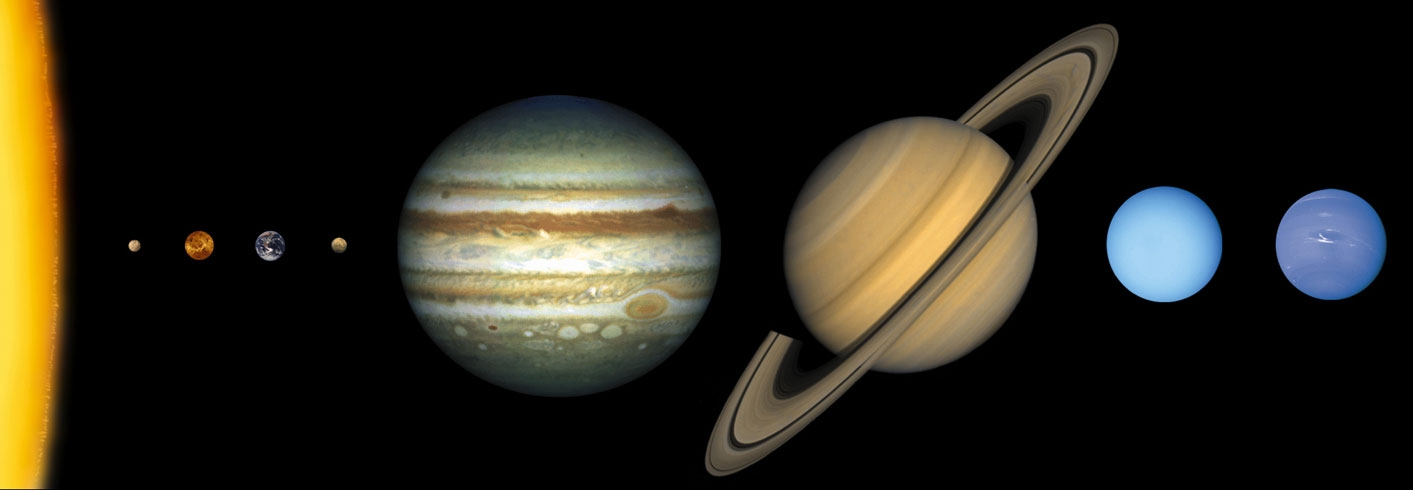
\includegraphics[width=0.9\textwidth{},keepaspectratio]{sun.jpg}
  \bicaption[fig:sun]{太阳系}{最左侧是太阳,向右依序为水星、金星、地球、火星、
    木星、土星、天王星与海王星}{Fig.}{Outward from the Sun, the planets
    are Mercury, Venus, Earth, Mars, Jupiter, Saturn, Uranus and
    Neptune.}
\end{figure}

\begin{table}[htbp]
  \bicaption[tab:xingxing]{行星数据表1}{行星数据表}{Tab.}{Planet}
  \centering
  \vspace{0.2cm}
  \zhongwu
  \begin{tabular}{cccc}
    \toprule
    Planet  & Size(Earth=1) & Weight(Earth=1) & Radius  \\
    \midrule
    Mercury & 0.056         & 0.055           & 0.3871  \\
    Venus   & 0.857         & 0.815           & 0.7233  \\
    Earth   & 1.00          & 1.000           & 1.0000  \\
    Mars    & 0.151         & 0.107           & 1.5237  \\
    Jupiter & 1321          & 317.832         & 5.2026  \\
    Saturn  & 755           & 95.16           & 9.5549  \\
    Uranus  & 63            & 14.54           & 19.2184 \\
    Neptune & 58            & 17.15           & 30.1104 \\
    \bottomrule
  \end{tabular}
\end{table}

表~\ref{tab:xingxing}的源代码如下:
\vspace{1em}
\begin{lstlisting}
  \begin{table}[htbp]
    \bicaption[tab:xingxing]{行星数据表1}{行星数据表}{Tab.}{Planet}
    \centering
    \vspace{0.2cm}
    \zhongwu
    \begin{tabular}{cccc}
      \toprule
      Planet  & Size(Earth=1) & Weight(Earth=1) & Radius  \\
      \midrule
      Mercury & 0.056         & 0.055           & 0.3871  \\
      Venus   & 0.857         & 0.815           & 0.7233  \\
      Earth   & 1.00          & 1.000           & 1.0000  \\
      Mars    & 0.151         & 0.107           & 1.5237  \\
      Jupiter & 1321          & 317.832         & 5.2026  \\
      Saturn  & 755           & 95.16           & 9.5549  \\
      Uranus  & 63            & 14.54           & 19.2184 \\
      Neptune & 58            & 17.15           & 30.1104 \\
      \bottomrule
    \end{tabular}
  \end{table}
\end{lstlisting}

表格和插图通常需要占据大块空间,所以在文字处理软件中用户经常需要调整它们的
位置。 \texttt{table}环境可以自动完成这样的任务,这种自动调整位置的环境称作
浮动环境 (float)\footnote{下一节里还会介绍插图浮动环境}。table环境是一个将表格嵌入文本的浮动环境。

\texttt{htbp} 选项用来指定表格的理想位置,这几个字母分别代表 here, top,
bottom,float page,也就是就这里、页顶、页尾、浮动页 (专门放浮动环境的单独
页面)。我们可以使用这几个字母的任意组合,四个字母都写上表示放哪里都无所
谓;一般不推荐单独使用h,因为 \LaTeX{}自以为它的排版算法是最完美的,不愿意
被束缚手脚。

\verb|\centering| 用来使表格居
中; \verb|\bicaption| 命令设置表格标题, \LaTeX{}会自动给
浮动环境的标题加上编号。

它的官方使用说明为:
\begin{lstlisting}
  \bicaption[label]{ 中文短标题 }{ 中文标题 }{Tab.}{ 英文标题 }
\end{lstlisting}
可选参数~label~用来作为交叉引用链接。例如
表~\ref{tab:xingxing}中的 lable为 tab:xingxing 。这里的标
签一般为英文。中文短标题一般没什么用,可以随意填。最简单就是“表”。

在表格环境中,标题必须位于表格的上方。而在图片环境中,标题的位置必须位于
图片的下方。

tabular 环境提供了最简单的表格功能。它用 \texttt{\&} 来分列,
用 \texttt{\textbackslash{\textbackslash{}}} 来换行;每列可以采用居中、居
左、居右等横向对齐方式,分别用 \texttt{l、c、r} 来表示。

三线表的三条横线就分别
用 \verb|\toprule、 \midrul、\bottomrule| 等命令表示。

\verb|\vspace{0.2cm}| 是用来控制表格标题与表格正文的
垂直间距的,请在插入表格时务必添加。 \verb|\zhongwu| 是
用来调整表格内容的行距的。


\subsection{多列三线表}

在三线表中,有些列的列头会横跨好几列的数据。一般使
用 \verb|\multicolumn| 命令。它的用法是:
\begin{lstlisting}
  \multicolumn{ 列数}{ 对齐方式 }{ 表格内容 }
\end{lstlisting}

“列数”是指这一列横跨的列数,在表~\ref{tab:linux}是2列,就填“2”;“对
齐方式”从\texttt{lcr}三者中选其一即可,在表~\ref{tab:linux}中是c。“表格
内容”填入自己的内容。一般还会在这一列的下面画一小横线,已示辨识。使
用 \verb|\cmidrule| 命令。在表~\ref{tab:linux}中,由于横跨的是第2列和第3列,
因此 \verb|\cmidrule| 的参数是2-3。

\begin{table}[htbp]
  \bicaption[tab:linux]{不同操作系统下的\LaTeX{}}{ 不同操作系统下的\LaTeX{} }{Tab.}{OS with \LaTeX{}}
  \centering
  \vspace{0.2cm}
  \zhongwu
  \begin{tabular}{ccc}
    \toprule
    Test    & \multicolumn{2}{c}{Common Tools} \\
              \cmidrule{2-3}
    OS         & Distribution & Editor  \\
    \midrule
    Windows    & MikTeX       & TexMakerX  \\
    Mac OS     & MacTeX       & TeXShop  \\
    Linux/Unix & TeX Live     & TeXworks  \\
    \bottomrule
  \end{tabular}
\end{table}


\begin{lstlisting}
  \begin{table}[htbp]
    \bicaption[tab:linux]{不同操作系统下的\LaTeX{}}{不同操作系统下的\LaTeX{}}
    {Tab.}{OS with \LaTeX{}}
    \centering
    \vspace{0.2cm}
    \zhongwu
    \begin{tabular}{ccc}
      \toprule
      Test    & \multicolumn{2}{c}{Common Tools} \\
                \cmidrule{2-3}
      OS         & Distribution & Editor  \\
      \midrule
      Windows    & MikTeX       & TexMakerX  \\
      Mac OS     & MacTeX       & TeXShop  \\
      Linux/Unix & TeX Live     & TeXworks  \\
      \bottomrule
    \end{tabular}
  \end{table}
\end{lstlisting}

\subsection{多行三线表}

既然有多列三线表,多行三线表也是用类似的方法解决。我们把表~\ref{tab:linux} 来改造一下,相对应的,一般使用 \verb|\multirow| 命令。它的用法
是:
\begin{lstlisting}
  \multirow{ 行数 }*{ 表格内容 }
\end{lstlisting}

“行数”是指竖向跨的行数,在表~\ref{tab:unix}中是2行,中间有个星号,表示自然宽度。

\begin{table}[htbp]
  \bicaption[tab:unix]{不同操作系统下的\LaTeX{}}{ 不同操作系统下的\LaTeX{} }{Tab.}{OS with \LaTeX{}}
  \centering
  \vspace{0.2cm}
  \zhongwu
  \begin{tabular}{ccc}
    \toprule
    \multirow{2}*{OS} & \multicolumn{2}{c}{Common Tools} \\
    \cmidrule{2-3}
    & Distribution & Editor  \\
    \midrule
    Windows          & MikTeX       & TexMakerX  \\
    Mac OS           & MacTeX       & TeXShop  \\
    Linux/Unix       & TeX Live     & TeXworks  \\
    \bottomrule
  \end{tabular}
\end{table}


\begin{lstlisting}
  \begin{table}[htbp]
    \bicaption[tab:unix]{不同操作系统下的\LaTeX{}}{不同操作系统下的\LaTeX{}}
    {Tab.}{OS with \LaTeX{}}
    \centering
    \vspace{0.2cm}
    \zhongwu
    \begin{tabular}{ccc}
      \toprule
      \multirow{2}*{OS} & \multicolumn{2}{c}{Common Tools} \\
      \cmidrule{2-3}
      & Distribution & Editor  \\
      \midrule
      Windows          & MikTeX       & TexMakerX  \\
      Mac OS           & MacTeX       & TeXShop  \\
      Linux/Unix       & TeX Live     & TeXworks  \\
      \bottomrule
    \end{tabular}
  \end{table}
\end{lstlisting}

\section{列宽可调表格的绘制方法}

论文中能用到列宽可调表格的情况共有两种,一种是当插入的表格某一单元格内容过长以至于一行放不下的情况,
另一种是当对公式中首次出现的物理量符号进行注释的情况,这两种情况都需要调用~tabularx~宏包。下面将分别对这两种情况下可调表格的绘制方法进行阐述。

\subsection{宽度控制}

有时候表格中的某行太长了,需要折行。可以使用\texttt{tabularx} 宏包的同名
环境,其语法如下:

\begin{lstlisting}
  \begin{tabularx}{ 表格总宽度 }{ 对齐方式 }
    ...
  \end{tabularx}
\end{lstlisting}

“表格总宽度”最好用\texttt{textwidth}乘以某个系数表示。例
如\texttt{0.8\textbackslash{textwidth}}表示表格宽度是版芯宽度的0.8倍。这
样出来的效果比较好看。对齐方式除了原有的\texttt{l,c,r}之外,多了一
个\texttt{X},表示某列可以折行。

\begin{table}[htbp]
  \centering
  \bicaption[tab:wall]{墙上的44句话}{墙上的44句话}{Tab.}{Mikko Kuorinki}
  \vspace{0.2cm}
  \zhongwu
  \begin{tabularx}{0.8\textwidth{}}{lX}
    \toprule
    People & Says \\
    \midrule
    Elias Canetti & If you were alone, you would cut yourself in two, so
    that one part would shape the other.\\
    Franz Kafka & In the struggle between yourself and the world,
    second the world.\\
    \bottomrule
  \end{tabularx}
\end{table}

\begin{lstlisting}
  \begin{table}[htbp]
    \centering
    \bicaption[tab:figure]{墙上的44句话}{墙上的44句话}{Tab.}{Mikko Kuorinki}
    \vspace{0.2cm}
    \zhongwu
    \begin{tabularx}{0.8\textwidth{}}{lX}
      \toprule
      People & Says \\
      \midrule Elias Canetti & If you were alone, you would cut yourself
      in two, so  that one part would shape the other.\\
      Franz Kafka & In the struggle between yourself and the world,
      second the world.\\
      \bottomrule
    \end{tabularx}
  \end{table}
\end{lstlisting}

\subsection{表格内某单元格内容过长的情况}

首先给出这种情况下的一个例子如表~\ref{table3}~所示。
\begin{table}[htbp]
  \centering
\bicaption[table3]{}{最小的三个正整数的英文表示法}{Table$\!$}{The English construction of the smallest three positive integral numbers}\vspace{0.5em}\wuhao
\begin{tabularx}{0.7\textwidth}{llX}
\toprule[1.5pt]
Value & Name & Alternate names, and names for sets of the given size\\\midrule[1pt]
1 & One & ace, single, singleton, unary, unit, unity\\
2 & Two & binary, brace, couple, couplet, distich, deuce, double, doubleton, duad, duality, duet, duo, dyad, pair, snake eyes, span, twain, twosome, yoke\\
3 & Three & deuce-ace, leash, set, tercet, ternary, ternion, terzetto, threesome, tierce, trey, triad, trine, trinity, trio, triplet, troika, hat-trick\\\bottomrule[1.5pt]
\end{tabularx}
\end{table}

绘制这种表格的代码及其说明如下。
\vspace{1em}
\begin{lstlisting}
\begin{table}[htbp]
\bicaption[标签名]{}{中文标题}{Table$\!$}{English caption}
\vspace{0.5em}\wuhao
\begin{tabularx}{\textwidth}{l...X...l}
\toprule[1.5pt]
表头第1个格   & ... & 表头第X个格   & ... & 表头第n个格  \\
\midrule[1pt]
表中数据(1,1) & ... & 表中数据(1,X) & ... & 表中数据(1,n)\\
表中数据(2,1) & ... & 表中数据(2,X) & ... & 表中数据(2,n)\\
.........................................................\\
表中数据(m,1) & ... & 表中数据(m,X) & ... & 表中数据(m,n)\\
\bottomrule[1.5pt]
\end{tabularx}
\end{table}
\end{lstlisting}


tabularx环境共有两个必选参数:第1个参数用来确定表格的总宽度,这里取为排版表格能达到的最大宽度——正文宽度 \verb|\textwidth| ;第2个参数用来确定每列格式,其中标为X的项表示该列的宽度可调,其宽度值由表格总宽度确定。
标为X的列一般选为单元格内容过长而无法置于一行的列,这样使得该列内容能够根据表格总宽度自动分行。若列格式中存在不止一个X项,则这些标为X的列的列宽相同,因此,一般不将内容较短的列设为X。
标为X的列均为左对齐,因此其余列一般选为l(左对齐),这样可使得表格美观,但也可以选为c或r。


\section{斜线表头}

还是有些童鞋的表示三线表不实用啊,非要回归到原来的斜线表头去。我们可以使
用宏包 diagbox 提供的命令轻松完成。不过呢,出来的表格很 ugly 罢了。

diagbox 是宏包提供的主要命令。它可以带有两个必选参数,表示要生成斜
线表头的两部分内容。默认斜线是从西北到东南方向的。

需要注意的是,使用斜线表格后就不能使用三线表的三条横线,不然请看
表~\ref{tab:diagbox}的下场。正确的做法是使用最原始的 hline,见
表~\ref{tab:xiexian}。

\begin{table}[htbp]
  \bicaption[tab:diagbox]{斜线表头}{斜线表头}{Tab.}{Diagbox}
  \centering
  \vspace{0.2cm}
  \zhongwu
  \begin{tabular}{|l|ccc|}
    \toprule
    \diagbox{Times}{Day} & Mon  & Tue  & Wed  \\
    \midrule
    Morning              & used & used &  \\
    Afternoon            &      & used & used \\
    \bottomrule
  \end{tabular}
\end{table}

\begin{lstlisting}
  \begin{table}[htbp]
    \bicaption[tab:diagbox]{斜线表头}{斜线表头}{Tab.}{Diagbox}
    \centering
    \vspace{0.2cm}
    \zhongwu
    \begin{tabular}{|l|ccc|}
      \toprule
      \diagbox{Times}{Day} & Mon  & Tue  & Wed  \\
      \midrule
      Morning              & used & used &  \\
      Afternoon            &      & used & used \\
      \bottomrule
    \end{tabular}
  \end{table}
\end{lstlisting}

\begin{table}[htbp]
  \bicaption[tab:xiexian]{斜线表头}{斜线表头}{Tab.}{Diagbox}
  \centering
  \vspace{0.2cm}
  \zhongwu
  \begin{tabular}{|l|ccc|}
    \hline
    \diagbox{Times}{Day} & Mon  & Tue  & Wed  \\
    \hline
    Morning              & used & used &  \\
    Afternoon            &      & used & used \\
    \hline
  \end{tabular}
\end{table}

\begin{lstlisting}
  \begin{table}[htbp]
    \bicaption[tab:xiexian]{斜线表头}{ 斜线表头 }{Tab.}{Diagbox}
    \centering
    \vspace{0.2cm}
    \zhongwu
    \begin{tabular}{|l|ccc|}
      \hline
      \diagbox{Times}{Day} & Mon  & Tue  & Wed  \\
      \hline
      Morning              & used & used &  \\
      Afternoon            &      & used & used \\
      \hline
    \end{tabular}
  \end{table}
\end{lstlisting}


\section{表格的列按小数点对齐}

以表~\ref{tab:xingxing}为例,想把其中的第三列按小数点对齐\footnote{参见宏
  包siunitx}。先看一下效果:

在表~\ref{tab:xiaoshu}中,我们调整了原来四列数的对齐方式。原来
是\texttt{cccc},现在是\texttt{lcSr}。第一列左对齐,第二列不变,还是居中
对齐,第四列右对齐。值得注意的是第三列,这里新引入了一个参数\texttt{S},
含义就是这一列的数字按照小数点对齐。一定是大写的S。另外,第三列的列
头Weight(Earth=1)两边也加上了大括号,因为这不是数字。在使用参
数\texttt{S}的时候,不是数字的行需要用大括号括起来,不然会造成编译错误。

\begin{table}[htbp]
  \bicaption[tab:xiaoshu]{行星数据表2}{行星数据表}{Tab.}{Planet}
  \centering
  \vspace{0.2cm}
  \zhongwu
  \begin{tabular}{lcSr}
    \toprule
    Planet  & Size(Earth=1) & {Weight(Earth=1)} & Radius  \\
    \midrule
    Mercury & 0.056         & 0.055           & 0.3871  \\
    Venus   & 0.857         & 0.815           & 0.7233  \\
    Earth   & 1.00          & 1.000           & 1.0000  \\
    Mars    & 0.151         & 0.107           & 1.5237  \\
    Jupiter & 1321          & 317.832         & 5.2026  \\
    Saturn  & 755           & 95.16           & 9.5549  \\
    Uranus  & 63            & 14.54           & 19.2184 \\
    Neptune & 58            & 17.15           & 30.1104 \\
    \bottomrule
  \end{tabular}
\end{table}

\begin{lstlisting}
  \begin{table}[htbp]
    \bicaption[tab:xiaoshu]{行星数据表}{行星数据表}{Tab.}{Planet}
    \centering
    \vspace{0.2cm}
    \zhongwu
    \begin{tabular}{lcSr}
      \toprule
      Planet  & Size(Earth=1) & {Weight(Earth=1)} & Radius  \\
      \midrule
      Mercury & 0.056         & 0.055           & 0.3871  \\
      Venus   & 0.857         & 0.815           & 0.7233  \\
      Earth   & 1.00          & 1.000           & 1.0000  \\
      Mars    & 0.151         & 0.107           & 1.5237  \\
      Jupiter & 1321          & 317.832         & 5.2026  \\
      Saturn  & 755           & 95.16           & 9.5549  \\
      Uranus  & 63            & 14.54           & 19.2184 \\
      Neptune & 58            & 17.15           & 30.1104 \\
      \bottomrule
    \end{tabular}
  \end{table}
\end{lstlisting}

\section{对物理量符号进行注释的情况}

为使得对公式中物理量符号注释的转行与破折号“——”后第一个字对齐,此处最好采用表格环境。此表格无任何线条,左对齐,
且在破折号处对齐,一共有“式中”二字、物理量符号和注释三列,表格的总宽度可选为文本宽度,因此应该采用\verb|tabularx|环境。
由\verb|tabularx|环境生成的对公式中物理量符号进行注释的公式如式(\ref{eq:1})所示。

\begin{equation}\label{eq:1}
\ddot{\boldsymbol{\rho}}-\frac{\mu}{R_{t}^{3}}\left(3\mathbf{R_{t}}\frac{\mathbf{R_{t}\rho}}{R_{t}^{2}}-\boldsymbol{\rho}\right)=\mathbf{a}
\end{equation}
\begin{tabularx}{\textwidth}{@{}l@{\quad}r@{——}X@{}}
式中& $\boldsymbol{\rho}$ &追踪飞行器与目标飞行器之间的相对位置矢量;\\
&  $\boldsymbol{\ddot{\rho}}$&追踪飞行器与目标飞行器之间的相对加速度;\\
&  $\mathbf{a}$   &推力所产生的加速度;\\
&  $\mathbf{R_t}$ & 目标飞行器在惯性坐标系中的位置矢量;\\
&  $\omega_{t}$ & 目标飞行器的轨道角速度;\\
&  $\mathbf{g}$ & 重力加速度,$=\frac{\mu}{R_{t}^{3}}\left(
3\mathbf{R_{t}}\frac{\mathbf{R_{t}\rho}}{R_{t}^{2}}-\boldsymbol{\rho}\right)=\omega_{t}^{2}\frac{R_{t}}{p}\left(
3\mathbf{R_{t}}\frac{\mathbf{R_{t}\rho}}{R_{t}^{2}}-\boldsymbol{\rho}\right)$,这里~$p$~是目标飞行器的轨道半通径。
\end{tabularx}
\vspace{\wordsep}

其中生成注释部分的代码及其说明如下。
\vspace{1em}
\begin{lstlisting}
\begin{tabularx}{\textwidth}{@{}l@{\quad}r@{— —}X@{}}
式中 & symbol-1 & symbol-1的注释内容;\\
     & symbol-2 & symbol-2的注释内容;\\
     .............................;\\
     & symbol-m & symbol-m的注释内容。
\end{tabularx}\vspace{\wordsep}
\end{lstlisting}


tabularx环境的第1个参数选为正文宽度,第2个参数里面各个符号的意义为:
    第1个 \@{}表示在“式中”二字左侧不插入任何文本,“式中”二字能够在正文中左对齐,若无此项,则“式中”二字左侧会留出一定的空白;
    \@{\quad}表示在“式中”和物理量符号间插入一个空铅宽度的空白;
    \@{— — —}实现插入破折号的功能,它由三个1/2的中文破折号构成;
    第2个 \@{}表示在注释内容靠近正文右边界的地方能够实现右对齐。


由此方法生成的注释内容应紧邻待注释公式并置于其下方,因此不能将代码放入\verb|table|浮动环境中。但此方法不能实现自动转页接排,
可能会在当前页剩余空间不够时,全部移动到下一页而导致当前页出现很大空白。因此在需要转页处理时,还请您手动将需要转页的代码放入一个
新的\verb|tabularx|环境中,将原来的一个\verb|tabularx|环境拆分为两个\verb|tabularx|环境。


\section{罗列}
学位论文一般可采用两种罗列环境:一种是并列条目有同样标签的~\verb|itemize|~罗列环境,另一种是具有自动排序编号符号的~\verb|enumerate|~罗列环境。这两种罗列环境的样式参数可参考图~\ref{list}。
\begin{figure}[htbp]
\centering
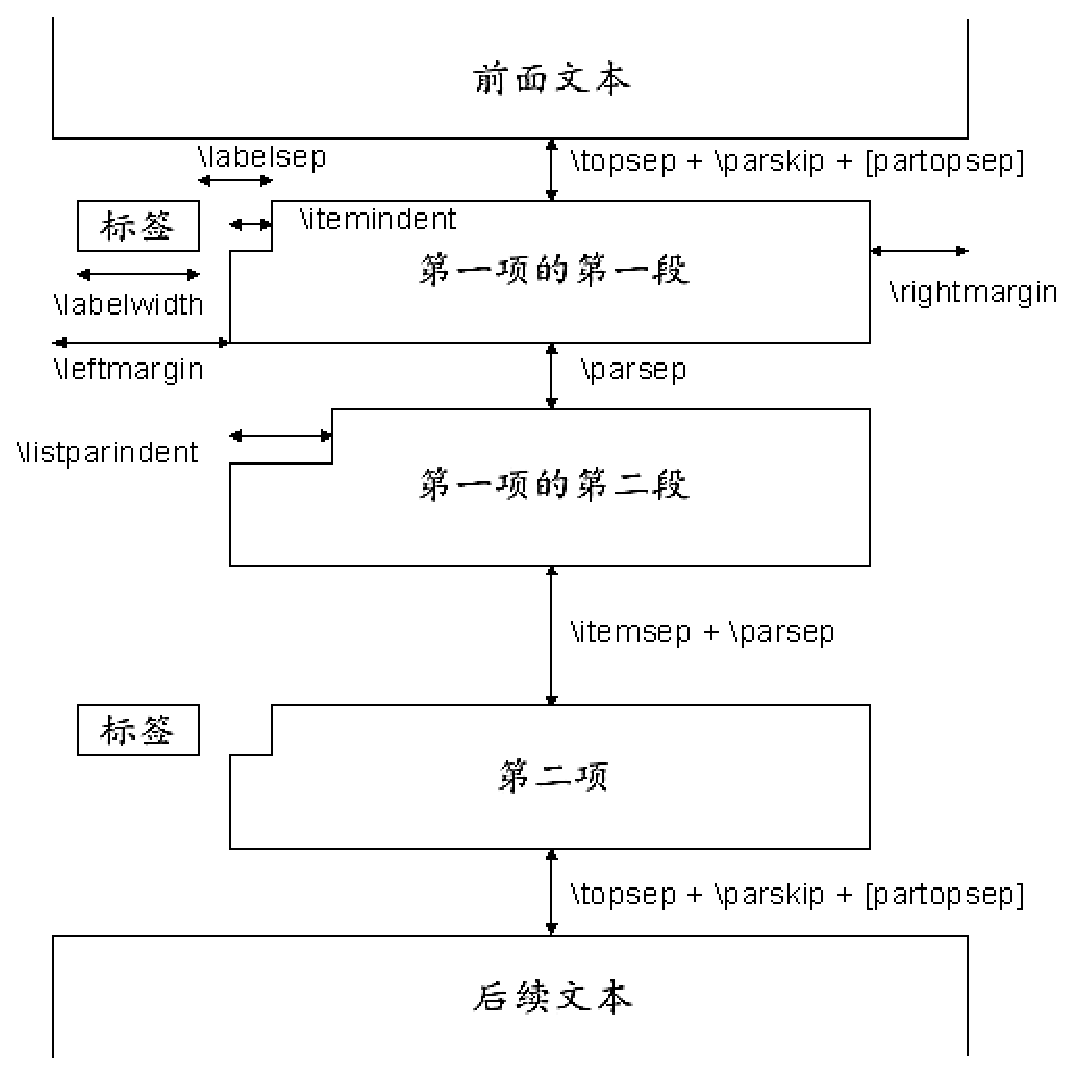
\includegraphics[width = 0.6\textwidth]{list}
\bicaption[list]{}{罗列环境参数示意图}{Fig.$\!$}{Schematic diagram of list environments}\vspace{-1em}
\end{figure}

通过调用~enumitem~宏包可以很方便地控制罗列环境的布局,其~format.tex~文件中的~\verb|\setitemize|~和~\verb|\setenumerate|~命令分别用来设置~\verb|itemize|~和~\verb|enumerate|~环境的样式参数。采用~\verb|itemize|~单层罗列环境的排版形式如下:

\begin{itemize}
\item 第一个条目文本内容
\item 第二个条目文本内容
\item 第三个条目文本内容
\end{itemize}

其代码如下
\begin{verbatim}
\begin{itemize}
  \item 第一个条目文本内容
  \item 第二个条目文本内容
  ...
  \item 第三个条目文本内容
\end{itemize}
\end{verbatim}

采用~\verb|enumerate|~单层罗列环境的排版形式如下:
\begin{enumerate}
\item 第一个条目文本内容
\item 第二个条目文本内容
\item 第三个条目文本内容
\end{enumerate}

其代码如下
\begin{verbatim}
\begin{enumerate}
  \item 第一个条目文本内容
  \item 第二个条目文本内容
  ...
  \item 第三个条目文本内容
\end{enumerate}
\end{verbatim}

例如:

\begin{enumerate}
\item 鉴定袋蛾———二十分
\item 给斯拉瓦写信———二小时四十五分
\item 植物保护小组开会———二小时二十五分
\end{enumerate}

上述是默认的列表样式。源代码如下:
\begin{lstlisting}
  \begin{enumerate}
  \item 鉴定袋蛾———二十分
  \item 给斯拉瓦写信———二小时四十五分
  \item 植物保护小组开会———二小时二十五分
  \end{enumerate}
\end{lstlisting}

\texttt{emumerate}环境就是罗列环境。每条\verb|\item| 后面
跟一个空格,然后就是具体的罗列条目。

默认的样式是按照(1),(2),(3)来排序的,如果想按照英文字母(a),(b),(c)或者罗
马数字(i),(ii),(iii)这样的顺序呢,只需要
在 \verb|\begin{enumerate}| 后面加一个参数,参数放在方括
号内。比如:
\begin{enumerate}[(a)]
\item 鉴定袋蛾———二十分
\item 给斯拉瓦写信———二小时四十五分
\item 植物保护小组开会———二小时二十五分
\end{enumerate}
源代码是:
\begin{lstlisting}
  \begin{enumerate}[(a)]
  \item 鉴定袋蛾———二十分
  \item 给斯拉瓦写信———二小时四十五分
  \item 植物保护小组开会———二小时二十五分
  \end{enumerate}
\end{lstlisting}

如上,方括号的中参数是可以更改的。a代表小写字母,A代表大写字母,1代表数
字,i代表小写罗马数字,I代表大写罗马数字。这些参数可以加上圆括号,也可以
加上一个点(英文句号)。\textcolor{red}{[a)]}:罗列的标签就会变
成a)、b)、c)。\textcolor{red}{[1.]}:罗列的标签就会变成1.、2.、3. 。

罗马数字的例子:
\begin{enumerate}[i.]
\item 鉴定袋蛾———二十分
\item 给斯拉瓦写信———二小时四十五分
\item 植物保护小组开会———二小时二十五分
\end{enumerate}
源代码:
\begin{lstlisting}
  \begin{enumerate}[i.]
  \item 鉴定袋蛾———二十分
  \item 给斯拉瓦写信———二小时四十五分
  \item 植物保护小组开会———二小时二十五分
  \end{enumerate}
\end{lstlisting}

\section*{本章小结}
表格和罗列排版方法介绍。

% !TEX TS-program = XeLaTeX
% !TEX encoding = UTF-8 Unicode

%%%%%%%%%%%%%%%%%%%%%%%%%%%%%%%%%%%%%%%%%%%%%%%%%%%%%%%%%%%%%%%%%%%%%%
%
%  哈尔滨工程大学学位论文 XeLaTeX 模版 —— 正文文件 chap04.tex
%
%  版本:1.0.0
%  最后更新:
%  修改者:Leo LiWenhui lwh@hrbeu.edu.cn
%  修订者:
%  编译环境1:Ubuntu 12.04 + TeXLive 2013/2014
%  编译环境2:Windows 7/8  + TeXLive 2013/2014
%
%%%%%%%%%%%%%%%%%%%%%%%%%%%%%%%%%%%%%%%%%%%%%%%%%%%%%%%%%%%%%%%%%%%%%

\chapter{插图}
\label{chap05}

\section{研究生院的插图规范}
图应有自明性。插图应与文字紧密配合,文图相符,内容正确。选图要力求精练,插图、照片应完整清晰。图中文字和数字等字号用宋体~5~号字。

机械工程图:采用第一角投影法,严格按照~GB4457---GB131-83《机械制图》标准规定。

数据流程图、程序流程图、系统流程图等按~GB1526-89~标准规定。

电气图:图形符号、文字符号等应符合附录~3~所列有关标准的规定。

流程图:必须采用结构化程序并正确运用流程框图。

对无规定符号的图形应采用该行业的常用画法。

坐标图的坐标线均用细实线,粗细不得超过图中曲线,有数字标注的坐标图,必须注明坐标单位。

照片图要求主题和主要显示部分的轮廓鲜明,便于制版。如用放大或缩小的复制品,必须清晰,反差适中。照片上应有表示目的物尺寸的标度。

引用文献图表必须标注出处。


\subsection{图题及图中说明}
每个图均应有图题(由图序和图名组成),图名在图序之后空一格排写。图序按章编排,如第~1~章第一个插图的图号为“图~1-1”等。
图题置于图下,硕士论文可只用中文书写,博士论文用中、英文两种文字居中书写,中文在上,要求中文用宋体~5~号字,英文用~Times New Roman 5~号字。有图注或其它说明时应置于图题之上。引用图应注明出处,在图题右上角加引用文献号。
图中若有分图时,分图题置于分图之下或图题之下,分图号用~a)、b)等表示。

图中各部分说明应采用中文(引用的外文图除外)或数字项号,各项文字说明置于图题之上(有分图题者,置于分图题之上)。

\subsection{插图编排}

插图之前,文中必须有关于本插图的提示,如“见图~1-1”、“如图~1-1~所示”等。插图与其图题为一个整体,不得拆开排写于两页。
插图处的该页空白不够排写该图整体时,则可将其后文字部分提前排写,将图移到次页。

\section{LaTeX~中推荐使用的图片格式}

论文使用的图片都放在figure文件夹中,图片可以是~EPS、JPG、PDF等格式。插图浮动环境是\texttt{figure},基本命
令是\texttt{includegraphics},而在图片环境中,标题的位置必须位于图片的下方。

\section{单张图片}

单张图片示例如图\ref{fig:wedding}所示。插入方法为插入浮动图后,在图片位置插入所需图片。一般需要使用段落设置将图形设置为居中,在图形两边插入水平填充也可实现居中。\textbackslash bicaption设置图形引用标识及图形标题,其格式为:

\begin{lstlisting}
\bicaption[fig:refname]{中文索引图名称}{中文图名称}{Eng_Index}{English Caption}
\end{lstlisting}

 引用图形时,需在图题处插入“图\textbackslash ref~\{fig:refname\}”,\LaTeX{}编译器会自动对插图序号进行编排,并用最终图号替换符号引用标识。

 如果图形图题过长,\LaTeX{}排版系统会自动按悬挂缩进排版。

\begin{figure}[htbp]
  \centering
  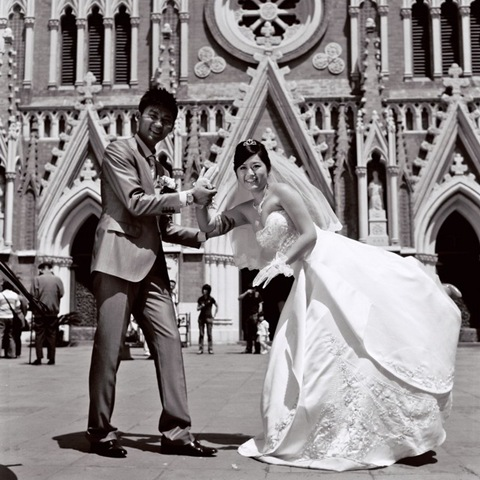
\includegraphics[scale=0.6]{wedding.jpg}
  \bicaption[fig:wedding]{婚礼}{婚礼}{Fig.}{Wedding}
\end{figure}

\begin{lstlisting}
  \begin{figure}[htbp]
    \centering
    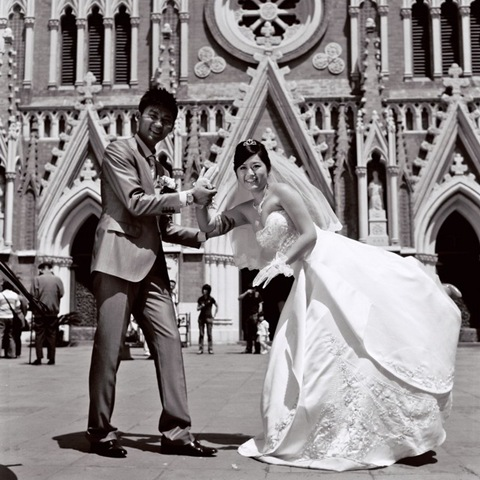
\includegraphics[scale=0.6]{wedding.jpg}
    \bicaption[fig:wedding]{婚礼}{婚礼}{Fig.}{Wedding}
  \end{figure}
\end{lstlisting}

\texttt{includegraphics}的基本参数见表~\ref{tab:figure}。

\begin{table}[htbp]
  \centering
  \bicaption[tab:figure]{插图命令参数}{插图命令参数}{Tab.}{Parameter}
  \vspace{0.2cm}
  \zhongwu
  \begin{tabularx}{0.8\textwidth{}}{lX}
    \toprule
    参数             & 说明 \\
    \midrule
    width=x,height=y & 宽度和高度,绝对尺寸,可用任意长度单位。  \\
    scale=s          & 缩放比。绝对尺寸和缩放比用一种即可,同时使用两者,绝对尺寸起作用。 \\
    keepaspectratio & 保持图形比例。宽度和高度通常设置一个即可,否则图形比
    例会失调,除非再加上此选 项,
    这样图形宽度和高度都不超过指定参数。     \\
    angle=a          & 逆时针旋转角度,单位是度。  \\
    \bottomrule
  \end{tabularx}
\end{table}

对于图~\ref{fig:wedding},只使用了\texttt{scale}这一个参数,缩放因子是0.6。
当然,也可以直接指定图形的宽度和高度。图~\ref{fig:sun}的源代码如下:

\begin{lstlisting}
  \begin{figure}[htbp]
    \centering
    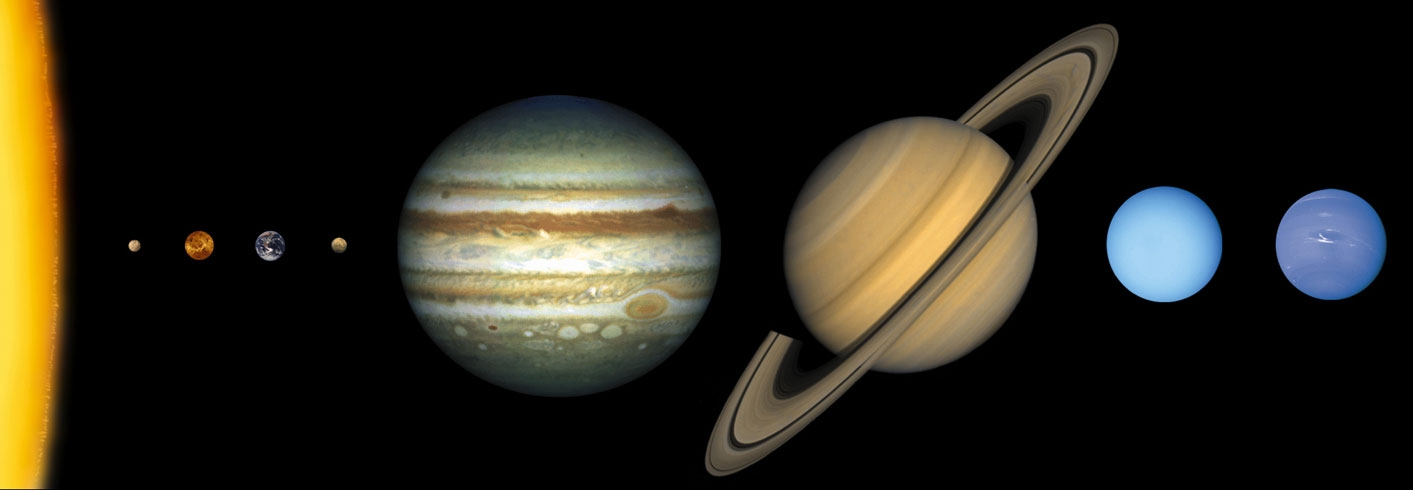
\includegraphics[width=\textwidth{},keepaspectratio]{sun.jpg}
    \bicaption[fig:sun]{太阳系}{最左侧是太阳,向右依序为水星、金
      星}{Fig.}{Outward from the Sun, the planets are Mercury, Venus,
      Earth, Mars, Jupiter, Saturn, Uranus and Neptune.}
  \end{figure}
\end{lstlisting}

可以看到,图~\ref{fig:sun}的宽度指定为版芯的宽度,然后使用了保持宽高比这
个选项。

\begin{figure}[tbph]
\usetikzlibrary{calc,through}
  \centering
    \begin{tikzpicture}
    \coordinate [label=left:$A$] (A) at (0,0);
    \coordinate [label=right:$B$] (B) at (0.75,0.25);
    \coordinate [label=above:$C$] (C) at (1,1.5);
    \draw (A) -- (B) -- (C);
    \coordinate [label=above:$D$] (D) at
    ($ (A) ! .5 ! (B) ! {sin(60)*2} ! 90:(B) $) {};
    \node (H) [label=135:$H$,draw,circle through=(C)] at (B) {};
    \draw (D) -- ($ (D) ! 3.5 ! (B) $) coordinate [label=below:$F$] (F);
    \draw (D) -- ($ (D) ! 2.5 ! (A) $) coordinate [label=below:$E$] (E);
    \end{tikzpicture}

    \bicaption[fig:sun]
    {长标题示例}
    {一个很长很长很长很长很长很长很长很长很长很长很长很长很长很长很长很长的标题示例
    这个图形是由Tikz绘制当然你也可以用JPG图片}
    {Fig.}
    {a long long long long long long long long long long long long caption}
\end{figure}

\begin{lstlisting}
\begin{figure}[tbph]
\usetikzlibrary{calc,through}
\centering
\begin{tikzpicture}
\coordinate [label=left:$A$] (A) at (0,0);
\coordinate [label=right:$B$] (B) at (0.75,0.25);
\coordinate [label=above:$C$] (C) at (1,1.5);
\draw (A) -- (B) -- (C);
\coordinate [label=above:$D$] (D) at
($ (A) ! .5 ! (B) ! {sin(60)*2} ! 90:(B) $) {};
\node (H) [label=135:$H$,draw,circle through=(C)] at (B) {};
\draw (D) -- ($ (D) ! 3.5 ! (B) $) coordinate [label=below:$F$] (F);
\draw (D) -- ($ (D) ! 2.5 ! (A) $) coordinate [label=below:$E$] (E);
\end{tikzpicture}

\bicaption[fig:sun]
{长标题示例}
{一个很长很长很长很长很长很长很长很长很长很长很长很长很长很长很长很长
的标题示例这个图形是由TikZ绘制当然你也可以用JPG图片}
{Fig.}
{a long long long long long long long long long long long long caption}
\end{figure}
\end{lstlisting}

长图题一般没有必要在插图目录中也完整显示,可使用菜单\texttt{Insert -{}-\textgreater{} Short
Title} 插入短标题 \verb|\index{ct\@插图\!dbt\@ 短标题} |。模板中已将图表编号两边设置了小的间距,不必再手动加入空格。


\section{双图并列}

并列图示例如图\ref{fig:lang}与图\ref{fig:niang}所示。

\begin{figure}[htbp]
  \centering
  \begin{minipage}{0.4\textwidth}
    \centering
    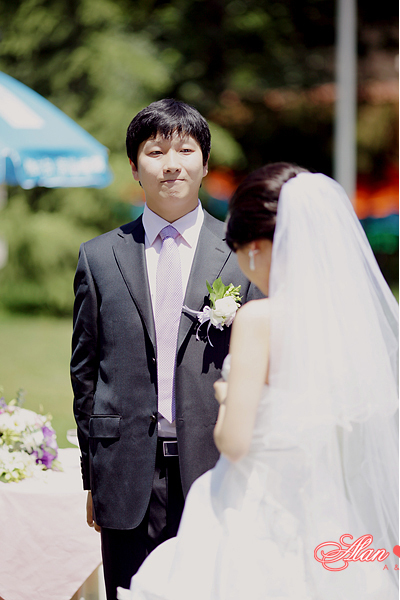
\includegraphics[keepaspectratio]{lang.jpg}
    \bicaption[fig:lang]{新郎}{新郎}{Fig.}{Bridegroom}
  \end{minipage}
  \begin{minipage}{0.4\textwidth}
    \centering
    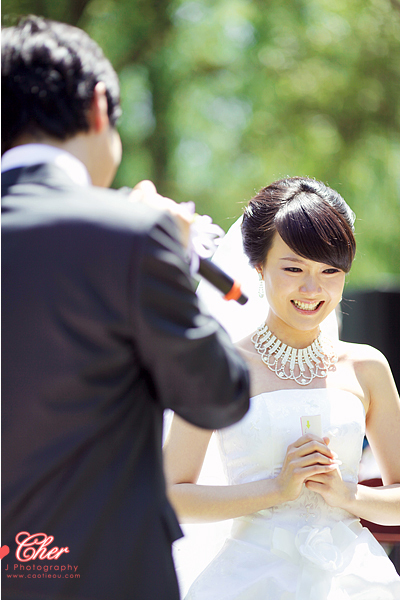
\includegraphics[keepaspectratio]{niang.jpg}
    \bicaption[fig:niang]{新娘}{新娘}{Fig.}{Brige}
  \end{minipage}
\end{figure}

\begin{lstlisting}
  \begin{figure}[htbp]
    \centering
    \begin{minipage}{0.4\textwidth}
      \centering
      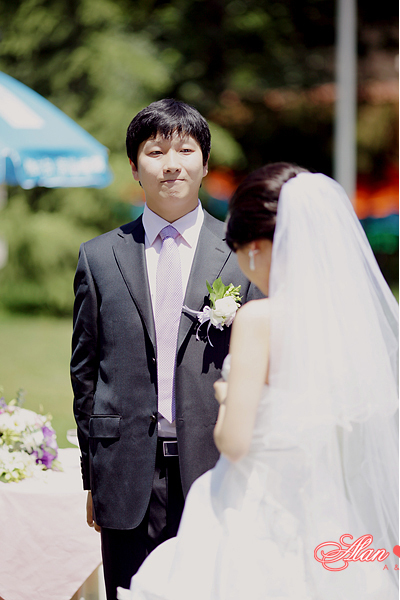
\includegraphics[keepaspectratio]{lang.jpg}
      \bicaption[fig:lang]{新郎}{新郎}{Fig.}{Bridegroom}
    \end{minipage}
    \begin{minipage}{0.4\textwidth}
      \centering
      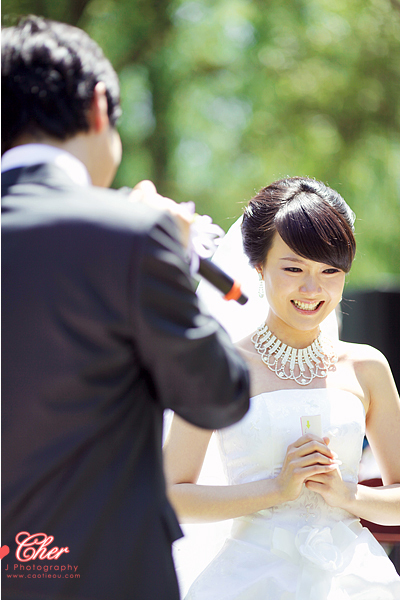
\includegraphics[keepaspectratio]{niang.jpg}
      \bicaption[fig:niang]{新娘}{新娘}{Fig.}{Brige}
    \end{minipage}
  \end{figure}
\end{lstlisting}

如果想要两幅并排的插图各有自己的标题,可以在 figure 环境中使用两
个 minipage 环境,每个里面插入一幅图 (见图~\ref{fig:lang}和
图~\ref{fig:niang}) 。不用 minipage 的话,因为插图标题的缺省宽度是
整个行宽;两幅插图就会上下排列。

这里指定了每个 minipage 的宽度为0.4倍的版芯宽度。当然,也可以自
己指定,只是两个宽度加起来不超过版芯宽度就可以了。

\section{两子图并列}

子图并列示例如图\ref{fig:judy}所示。

\begin{figure}[htbp]
    \centering
    \subfigure{\label{{fig:1a}}}\addtocounter{subfigure}{-2}
    \subfigure[Girl A]{\subfigure[女孩A]{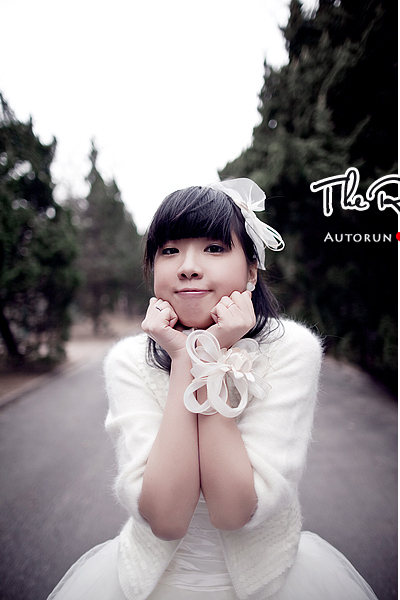
\includegraphics[keepaspectratio]{chao.jpg}}}
    \hspace{20pt}
    \subfigure{\label{{fig:1b}}}\addtocounter{subfigure}{-2}
    \subfigure[Girl B]{\subfigure[女孩B]{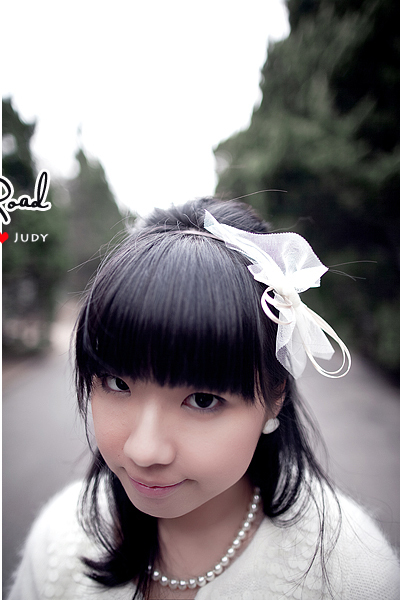
\includegraphics[keepaspectratio]{ren.jpg}}}
    \bicaption[fig:judy]{女孩}{女孩}{Fig.}{Judy}
\end{figure}

\begin{lstlisting}
  \begin{figure}[htbp]
    \centering
    \subfigure{\label{{fig:1a}}}\addtocounter{subfigure}{-2}
    \subfigure[Girl A]{\subfigure[女孩A]{
        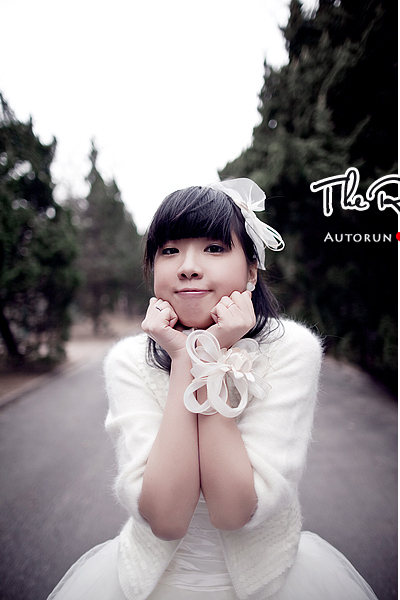
\includegraphics[keepaspectratio]{chao.jpg}}
    }
    \hspace{20pt}
    \subfigure{\label{{fig:1b}}}\addtocounter{subfigure}{-2}
    \subfigure[Girl B]{\subfigure[女孩B]{
        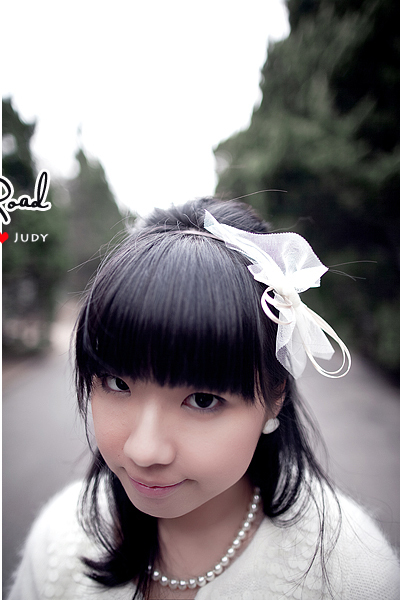
\includegraphics[keepaspectratio]{ren.jpg}}
    }
    \bicaption[fig:judy]{女孩}{女孩}{Fig.}{Judy}
  \end{figure}
\end{lstlisting}


如果想要两幅并排的图片共享一个标题,并且各有自己的子标题,学位论文规范要求不止总图的标题为中英文形式,其各个子图也应具有中英文形式的标题。
然而~ccaption~宏包却无法实现子图的中英文标题功能,这里采用对 \verb|\subfigure| 命令进行嵌套的方法来实现子图的中英文标题功能。如图~\ref{fig:judy},子图的标题用命令 \verb|\subcaption| 即可。
学位论文规范要求不止总图的标题为中英文形式,其各个子图也应具有中英文形式的标题。
然而~ccaption~宏包却无法实现子图的中英文标题功能,这里采用对 \verb|\subfigure| 命令进行嵌套的方法来实现子图的中英文标题功能


\section{pgf/TikZ~插图}
pgf/TikZ是一个在tex系统中的画图宏包,除了可以精确的作图外,对于某些不要求精确控制的图形绘制,如:流程图,树图,等等,也提供了简便易用的支持。
下面这张图片是用TikZ宏包进行绘制的图形,其实现代码为:
\begin{lstlisting}
    \begin{tikzpicture}[thick,smooth,domain=0:4,scale=0.9]
        \draw[very thin,gray] (0,0) grid (12,4);
        \draw plot[mark=*] (\x,{\x * \x/4});
        \draw[blue,xshift=4cm] plot[samples=5,mark=+] (\x,{\x * \x/4});
        \draw[red,xshift=8cm] plot[samples=10,mark=x] (\x,{\x * \x/4});
    \end{tikzpicture}
\end{lstlisting}

\begin{figure}[htbp]
    \centering
    \begin{tikzpicture}[thick,smooth,domain=0:4,scale=0.9]
        \draw[very thin,gray] (0,0) grid (12,4);
        \draw plot[mark=*] (\x,{\x * \x/4});
        \draw[blue,xshift=4cm] plot[samples=5,mark=+] (\x,{\x * \x/4});
        \draw[red,xshift=8cm] plot[samples=10,mark=x] (\x,{\x * \x/4});
    \end{tikzpicture}
  \bicaption[fig:TikZ]{TikZ插图}{TikZ插图}{Fig.}{Draw with TikZ}
\end{figure}

更多的关于pgf/TikZ请参考相关资料。

\section*{本章小结}
插图方法介绍。

% !TEX TS-program = XeLaTeX
% !TEX encoding = UTF-8 Unicode

%%%%%%%%%%%%%%%%%%%%%%%%%%%%%%%%%%%%%%%%%%%%%%%%%%%%%%%%%%%%%%%%%%%%%%
%
%  哈尔滨工程大学学位论文 XeLaTeX 模版 —— 正文文件 chap04.tex
%
%  版本:1.0.0
%  最后更新:
%  修改者:Leo LiWenhui lwh@hrbeu.edu.cn
%  修订者:
%  编译环境1:Ubuntu 12.04 + TeXLive 2013/2014
%  编译环境2:Windows 7/8  + TeXLive 2013/2014
%
%%%%%%%%%%%%%%%%%%%%%%%%%%%%%%%%%%%%%%%%%%%%%%%%%%%%%%%%%%%%%%%%%%%%%

\chapter{数学公式的排版}
\label{chap06}

\section{研究生院的公式规范}

论文中的公式应另起行,原则上应居中书写,与周围文字留有足够的空间区分开。
若公式前有文字(如“解”、“假定”等),文字空两格写,公式仍居中写。公式末不加标点。

公式应标注序号,并将序号置于括号内。 公式序号按章编排,如第~1~章第一个公式序号为“(1-1)”。公式的序号右端对齐。

公式较长时最好在等号“=”处转行,如难实现,则可在~$+$、$-$、$\times$、$\div$~运算符号处转行,转行时运算符号仅书写于转行式前,不重复书写。

文中引用公式时,一般用“见式~(1-1)”或“由公式~(1-1)”。

公式中用斜线表示“除”的关系时应采用括号,以免含糊不清,如~$a/(b\cos x)$。通常“乘”的关系在前,如~$a\cos x/b$而不写成~$(a/b)\cos x$。

不能用文字形式表示等式,如:$\textnormal{刚度}=\frac{{\textnormal{受力}}}{{\textnormal{受力方向的位移}}}$。

\textbf{对于数学公式的输入方法,网络上有一个比较全面权威的文档~\href{http://tug.ctan.org/cgi-bin/ctanPackageInformation.py?id=voss-mathmode}{Math mode}~请大家事先大概浏览一下。下面将对学位论文中主要用到的数学公式排版形式进行阐述。}

\section{生成~LaTeX~数学公式的两种方法}

对于先前没有接触过~\LaTeX~的人来说,编写~\LaTeX~数学公式是一件很繁琐的事,尤其是对复杂的数学公式来说,更可以说是一件难以完成的任务。
实际上,生成~\LaTeX~数学公式有一种基于~MathType~数学公式编辑器的简便方法。

MathType~是一款功能强大的数学公式编辑器软件,能够用来在文本环境中插入~Windows OLE~图形格式的复杂数学公式,所以应用比较普遍。但此软件只有~30~天的试用期,之后若再继续使用则需要付费购买才行。网络上有很多破解版的~MathType~软件可供下载免费使用,
笔者推荐下载安装版本号在~6.5~之上的中文破解版。

在安装好~MathType~之后,若在输入窗口中编写数学公式,复制到剪贴板上的仍然是图形格式的对象。
若希望得到可插入到~\LaTeX~编辑器中的文本格式对象,则需要对~MathType~软件做一下简单的设置:在~MathType~最上排的按钮中依次选择“参数选项
$\to$转换”,在弹出的对话窗中选中“转换到其它语言(文字):”,在转换下拉框中选择“Tex~--~--~LaTeX 2.09 and later”,并将对话框最下方的两个复选框全部勾掉,点击确定,这样,再从输入窗口中复制出来的对象就是文本格式的了,就可以直接将其粘贴到~\LaTeX~
编辑器中了。按照这种方法生成的数学公式两端分别有标记\verb|\[|和标记\verb|\]|,在这两个标记之间才是真正的数学公式代码。

若希望从~MathType~输入窗口中复制出来的对象为图形格式,则只需再选中“公示对象(Windows OLE~图形)”即可。


\section{行内公式}

出现在正文一行之内的公式称为行内公式,例如~$f(x)=\int_{a}^{b}\frac{\sin{x}}{x}\mathrm{d}x$。对于非矩阵和非多行形式的行内公式,一般不会使得行距发生变化,而~word~等软件却会根据行内公式的竖直距离而自动调节行距,如图~\ref{hangju}~所示。
\begin{figure}[htbp]
\centering
\subfigure{\label{latex}}\addtocounter{subfigure}{-2}
\subfigure[Inline mode equation derived from \LaTeX system]{\subfigure[由~\LaTeX~系统生成的行内公式]
          {\fbox{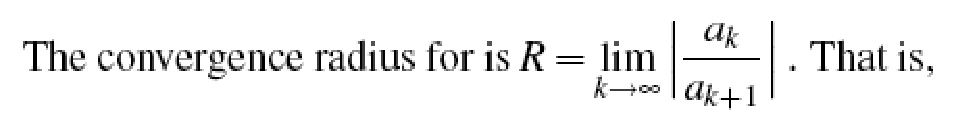
\includegraphics[width=0.55\textwidth]{latex}}}}
\subfigure{\label{word}}\addtocounter{subfigure}{-2}
\subfigure[Inline mode equation displayed as .doc format file derived from word software]{\subfigure[由~word软件生成的~.doc~格式行内公式]
          {\fbox{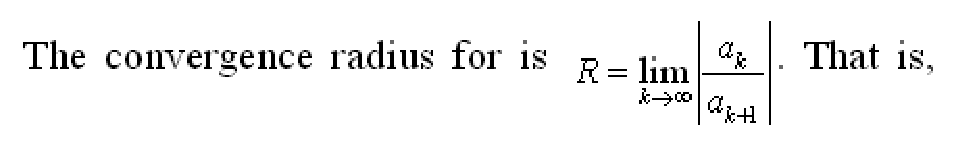
\includegraphics[width=0.55\textwidth]{word}}}}
\subfigure{\label{pdf}}\addtocounter{subfigure}{-2}
\subfigure[Inline mode equation displayed as .pdf format file derived from word software]{\subfigure[由~word软件生成的~.pdf~格式行内公式]
          {\fbox{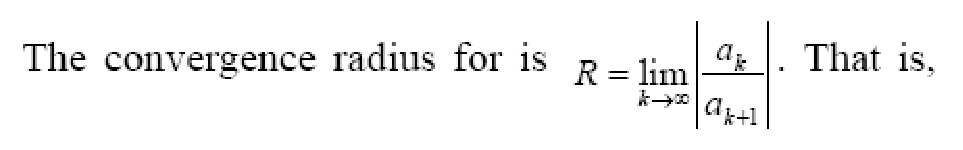
\includegraphics[width=0.55\textwidth]{pdf}}}}
\bicaption[hangju]{}{由~\LaTeX~和~word~生成的~3~种行内公式屏显效果}{Fig.$\!$}{Three kinds of inline mode equation displayed effects derived from \LaTeX and word}
\vspace{-1em}
\end{figure}
这三幅图分别为~\LaTeX~和~word~生成的行内公式屏显效果,从图中可看出,在~\LaTeX~文本含有公式的行内,在正文与公式之间对接工整,行距不变;而在~word~文本含有公式的行内,在正文与公式之间对接不齐,行距变大。因此从这一点来说,
\LaTeX~系统在数学公式的排版上具有很大优势。

\LaTeX~提供的行内公式最简单、最有效的方法是采用~\TeX~本来的标记——开始和结束标记都写作~\$,例如本节开始的例子可由下面的输入得到。
\begin{lstlisting}
  $f(x)=\int_{a}^{b}\frac{\sin{x}}{x}\mathrm{d}x$
\end{lstlisting}

\section{行间公式}

位于两行之间的公式称为行间公式,每个公式都是一个单独的段落,例如
\[\int_a^b{f\left(x\right)\mathrm{d}x}=\lim_{\left\|\Delta{x_i}\right\|\to 0}\sum_i{f\left(\xi_i\right)\Delta{x_i}}\]
除人工编号外,\LaTeX~各种类型行间公式的标记见表~\ref{eqtag}。
\begin{table}[htbp]
\bicaption[eqtag]{}{各种类型行间公式的标记}{Table$\!$}{Tags for several kinds of displaymath mode equations}
\vspace{0.5em}\centering\wuhao
\begin{tabularx}{0.9\textwidth}{cXX}
\toprule
& 无编号 & 自动编号\\\midrule
单行公式 & \textbackslash begin\{displaymath\}...... \textbackslash end\{displaymath\}~或~\textbackslash [...\textbackslash ] & \textbackslash begin\{equation\} ...... \textbackslash end\{equation\}\\
多行公式 & \textbackslash begin\{eqnarray*\} ...... \textbackslash end\{eqnarray*\} & \textbackslash begin\{eqnarray\} ...... \textbackslash end\{eqnarray\}\\
\bottomrule
\end{tabularx}
\end{table}
另外,在自动编号的某行公式行尾添加标签~\verb|\nonumber|,可将该行转换为无编号形式。

行间多行公式需采用~\verb|eqnarray|~或~\verb|eqnarray*|~环境,它默认是一个列格式为~\verb|rcl|~的~3~列矩阵,并且中间列的字号要小一些,因此通常只将需要对齐的运算符号(通常为等号“=”)置于中间列。

\section{可自动调整大小的定界符}

若在左右两个定界符之前分别添加命令~\verb|\left|~和~\verb|\right|,则定界符可根据所包围公式大小自动调整其尺寸,这可从式(\ref{nodelimiter})和式(\ref{delimiter})中看出。
\begin{equation}\label{nodelimiter}
(\sum_{k=\frac12}^{N^2})
\end{equation}
\begin{equation}\label{delimiter}
\left(\sum_{k=\frac12}^{N^2}\right)
\end{equation}
式(\ref{nodelimiter})和式(\ref{delimiter})是在~\LaTeX~中分别输入如下代码得到的。
\begin{lstlisting}
(\sum_{k=\frac12}^{N^2})
\left(\sum_{k=\frac12}^{N^2}\right)
\end{lstlisting}
\verb|\left|~和~\verb|\right|~总是成对出现的,若只需在公式一侧有可自动调整大小的定界符,则只要用“.”代替另一侧那个无需打印出来的定界符即可。

若想获得关于此部分内容的更多信息,可参见~\href{http://tug.ctan.org/cgi-bin/ctanPackageInformation.py?id=voss-mathmode}{Math mode}~文档的第~8~章“Brackets, braces and parentheses”。

\section{数学重音符号}

数学重音符号通常用来区分同一字母表示的不同变量,输入方法如下(需要调用~\verb|amsmath|~宏包):

\vspace{0.5em}\noindent\wuhao\begin{tabularx}{\textwidth}{Xc|Xc|Xc}
 \verb|\acute| & $\acute{a}$ & \verb|\mathring| & $\mathring{a}$ & \verb|\underbrace| & $\underbrace{a}$ \\
 \verb|\bar| & $\bar{a}$ & \verb|\overbrace| & $\overbrace{a}$ & \verb|\underleftarrow| & $\underleftarrow{a}$ \\
 \verb|\breve| & $\breve{a}$ & \verb|\overleftarrow| & $\overleftarrow{a}$ & \verb|\underleftrightarrow| & $\underleftrightarrow{a}$ \\
 \verb|\check| & $\check{a}$ & \verb|\overleftrightarrow| & $\overleftrightarrow{a}$ & \verb|\underline| & $\underline{a}$ \\
 \verb|\dddot| & $\dddot{a}$ & \verb|\overline| & $\overline{a}$ & \verb|\underrightarrow| & $\underrightarrow{a}$ \\
 \verb|\ddot| & $\ddot{a}$ & \verb|\overrightarrow| & $\overrightarrow{a}$ & \verb|\vec| & $\vec{a}$ \\
 \verb|\dot| & $\dot{a}$ & \verb|\tilde| & $\tilde{a}$ & \verb|\widehat| & $\widehat{a}$ \\
 \verb|\grave| & $\grave{a}$ & \verb|\underbar| & $\underbar{a}$ & \verb|\widetilde| & $\widetilde{a}$ \\
 \verb|\hat| & $\hat{a}$
\end{tabularx}\vspace{0.5em}
\xiaosi 当需要在字母~$i$~和~$j$~的上方添加重音符号时,为了去掉这两个字母顶上的小点,这两个字母应该分别改用~\verb|\imath|~和~\verb|\jmath|。

如果遇到某些符号不知道该采用什么命令能输出它时,则可通过~\href{http://detexify.kirelabs.org/classify.html}{Detexify$^2$~网站}来获取符号命令。若用鼠标左键在此网页的方框区域内画出你所要找的符号形状,则会在网页右方列出和你所画符号形状相近的~5~个符号及其相对应的~\LaTeX~输入命令。若所列出的符号中不包括你所要找的符号,还可通过点击“Select from the complete list!”的链接以得分从低到高的顺序列出所有符号及其相对应的~\LaTeX~输入命令。

最后,建议大家还是要以~\href{http://tug.ctan.org/cgi-bin/ctanPackageInformation.py?id=voss-mathmode}{Math mode}~这篇~pdf~文档作为主要参考。若要获得最为标准、美观的数学公式排版形式,可以查查文档中是否有和你所要的排版形式相同或相近的代码段,通过修改代码段以获得你所要的数学公式排版形式。

\section{数学公式排版示例}

下面是采用~\LaTeX~实现的几个简单的数学公式排版。

这是两个采用行内格式的数学公式,行内数学公式不带编号:

$f(x) = 3x + 7$

$$\sum_{i=1}^n a_i=0$$

下面是几个采用行间格式排版的数学公式,行间数学公式在最右侧自动编号:

\begin{definition}
  任给集合~$X \in U$ 和属性集~$R$, 对~$0\leqslant l < u \leqslant 1$,
  集合~$X$ 的~$l${--}下近似、$u${--}上近似分别定义为
     \begin{align}
\underline {R} _u (X) &=  \bigcup \left\{ {X_i  \in U/R\Bigm|X_i \mathop  \subseteq \limits^u  X} \right\}, \\
\overline {R} _l (X)  &=  \bigcup \left\{ {X_i  \in U/R\Bigm|X_i \mathop  \subset \limits^l X} \right\}.
   \end{align}
\end{definition}

\begin{theorem}[\hei 费马]
  {\upshape\kai 不存在使得~
  \begin{equation}
     x^n+y^n=z^n
  \end{equation}
  成立的整数~$x$, $y$, $z$ and $n>2$. }
\end{theorem}

\begin{proof}
  {\upshape\kai 这是推论
  \begin{equation}
     \textcolor[rgb]{0.00,0.00,1.00}{
     I'_{{\rm{total}}} = \sum\limits_{i = 1}^n
     {\left( {M_0 V_i - M_{i{\rm{rp}}} \sqrt{V_i^2 - V_{50}^2}}\right)}}
  \end{equation}}
\end{proof}

下面是一个稍微一些复杂的公式:

 \begin{equation}
{\mu _X}\sigma _X^2\sum\limits_{i = 1}^n {{{({X_i} - \bar X)}^2}} \frac{{x - \mu }}{\sigma }\frac{{{\partial ^2}\Omega }}{{\partial u\partial v}}\mathop{{\int\!\!\!\!\!\int\!\!\!\!\!\int}\mkern-31.2mu \bigodot}\nolimits_{x \in }
 {\bigcup\limits_{i = 1}^n {{X_i}} \frac{{dy}}{{dx}}}
\end{equation}

 利用~\LaTeX~你可以排出专业的数学版面效果。

\section*{本章小结}
数学公式排版方法介绍。

% !TEX TS-program = XeLaTeX
% !TEX encoding = UTF-8 Unicode

%%%%%%%%%%%%%%%%%%%%%%%%%%%%%%%%%%%%%%%%%%%%%%%%%%%%%%%%%%%%%%%%%%%%%%
%
%  哈尔滨工程大学学位论文 XeLaTeX 模版 —— 正文文件 chap04.tex
%
%  版本:1.0.0
%  最后更新:
%  修改者:Leo LiWenhui lwh@hrbeu.edu.cn
%  修订者:
%  编译环境1:Ubuntu 12.04 + TeXLive 2013/2014
%  编译环境2:Windows 7/8  + TeXLive 2013/2014
%
%%%%%%%%%%%%%%%%%%%%%%%%%%%%%%%%%%%%%%%%%%%%%%%%%%%%%%%%%%%%%%%%%%%%%

\chapter{参考文献}
\label{chap07}

参考文献的引用一般有两种方式,即行间引用和上标引用。

行间引用使用\textbackslash lcite~\{~~\}~语句实现,其显示效果是这样的:例如文献\lcite{DXM2005}论述了什么什么,而文献\lcite{OJP1999,kelton2002,strawderman2001,LQL1999}则对这个那个进行了研究。

上标引用使用\textbackslash cite~\{~~\}~语句实现,下面这段文字是普通的上标引用格式

我们的一切知识都是从经验开始\cite{LQL1999},这是没有任何怀疑的\cite{DXM2005}\cite{DXM2000};
因为,如果不是对象激动我们的感官,一则由它们自己引起表象,一则使我们的知性活动运作起来,对这些表象加
以比较,把它们粘结或分开,\cite{OJP1999,OJP1991}这样把感性印象的原始素材加工成称之为经验的对象
知识,那么知识能力又该由什么来唤起活动呢?\cite{braun2007,kelton2002,strawderman2001,LQL1999}所以
按照时间,我们没有任何知识是先行于经验的,一切知识都是从经验开始的。

只要是中文文献,图书,期刊,会议,专利等等需要为每个条目增加一个域:
\begin{lstlisting}
  language={CN},
\end{lstlisting}

对于\cite{DXM2005}参考文献\cite{OJP1999},原先的bib文件是\scite{OJP1991}这样的:
\begin{lstlisting}
  @article{ LQL1999 ,
    title={ 康德何以步安瑟尔谟的后尘? },
    author={ 李秋零 },
    journal={ 中国人民大学学报 },
    volume={2},
    year={1999}
  }
\end{lstlisting}


但是由于是中文文献,需要增加一个语言域,就变成下列样式:
\begin{lstlisting}
  @article{ LQL1999,
    title={ 康德何以步安瑟尔谟的后尘? },
    author={ 李秋零 },
    language={CN},
    journal={ 中国人民大学学报 },
    volume={2},
    year={1999}
  }
\end{lstlisting}

\section{~BibTeX~文献文件的写法}

用在~\LaTeX~中的~\textsc{Bib}\kern-.08em\TeX~文献文件的扩展名为~bib,此模板中,该文件即为~reference.bib。bibtex.exe 命令根据~GBT7714-2005NLang-HIT.bst 文件定义的文献格式,将~reference.bib 中的文献数据转换为输出文档中的文献列表。GBT7714-2005NLang-HIT.bst 文件是在~\href{http://bbs.ctex.org/attachment.php?aid=MjA3MDh8ZDcyMjc2MTN8MTMyNTYzNjY4OHxhZTg4bkNCUVJiRzA0WmU3TmlMbVdTUVExa0xtV2puWWc0dkdqbVJhbTVMdy9mVQ\%3D\%3D}{GBT7714-2005NLang-UTF8.bst} 文件的基础上修改得到的,所做的唯一一处改动是将姓氏字母全部大写的英文作者名改为只首字母大写,以保证和\href{http://219.217.226.141/xuewei/guifan.doc}{《研究生学位论文撰写规范》}及其\href{http://219.217.226.141/xuewei/fanli.doc}{《研究生学位论文书写范例》}相一致。

bib 文件的编写方法可参考模板中已给出的例子,也可参考~\href{http://bbs.ctex.org/attachment.php?aid=MTk3OTd8NjY1ODc5OGV8MTMyNTY0MTEyMnxhZGZkYWpsa0I2RGZwNDR5Z1lyeStjb1dKRS8rTnJub3lvT2FkNDNJbHl1UWVkVQ\%3D\%3D}{GBT7714-2005.bst 说明文档20060919
} 中所给出的例子。

中文文献需要添加一个额外的~language 域,并使得域值非空,这样~bst 文件就能够判断此文献为中文文献,进而能正确地生成参考文献格式。

GBT7714-2005.bst 对于国标~GB/T 7714-2005 的文献分类如表~\ref{tab:entrytypes} 所示。对于每种文献类型的缺省类型,已经设置好相应的文献标识码,因此不需要输入相应的文献
标识码。扩展类型的文献则应再添加一个~TypeofLit 域,并需要将其域值改为相应的文献标识码。
\begin{table}[htbp]
\bicaption[tab:entrytypes]{}{GBT7714-2005.bst 的分类方式}{Table$\!$}{Classification method of GBT7714-2005.bst}
\vspace{0.5em}\centering\wuhao
\begin{tabular}{llll}
\toprule[1.5pt]
文献类型 & 缺省类型 & 扩展类型(需要手 & 主要特征\\
 &  & 工加入文献标识码) & \\
\midrule[1pt]
article & 文章[J] & 报纸中的析出文献[N] & 年,卷(期):页码\\
 &  & 在线文章[J/OL] & \\
book & 书[M] & 论文集、会议录[C] & \\
 &  & 在线书[M/OL] & \\
 &  & 汇编[G] & \\
inbook & 书的某几页[M] &  & \\
incollection & 书中析出的文章[M]// & 汇编的析出文献[G]// & 析出文献[文献标识码]//\\
 &  & 标准的析出文献[S]// & \\
proceedings &  &  & \\
inproceedings & 论文集、会议录中的 & 在线论文集、 & 析出文献[文献标识码]//\\
/conference & 析出文献[C]// & 会议录[C/OL]// & \\
mastersthesis & 毕业论文[D] &  & 类似book类\\
phdthesis & 毕业论文[D] &  & 类似book类\\
techreport & 科技报告[R] &  & 类似book类\\
misc &  & 杂项[],例如:专利[P] & 此类一般是网上文件,\\
 &  & 网上专利[P/OL] & 按照国标规定顺序\\
 &  & 网上电子公告[EB/OL] & 编码制时不输出年份\\
 &  & 磁盘[CP/DK] & \\
\bottomrule[1.5pt]
\end{tabular}
\end{table}

《研究生学位论文撰写规范》及《研究生学位论文书写范例》中所列英文参考文献例子中的文章名的每个实词首字母都大写,因此需要将英文参考文献的~title 域手动修改为每个实词首字母大写。

英文参考文献在~author 域中的作者名需要将姓置前,名置后。

\section{参考文献的引用}

需要将~main.tex 文件中的语句~\verb|\nocite{*}| 屏蔽掉,这样,文中未引用的参考文献就不会出现在文后的参考文献列表中。文中参考文献的引用方法:

\begin{itemize}
\item 行文引用请使用命令~\verb|\lcite{引用词}|,引用效果为“\lcite{OJP1999}”;
\item 上标引用请使用命令~\verb|\cite{引用词}|,引用效果为“\cite{OJP1999}”。
\end{itemize}
其中,上标引用命令~\verb|\lcite{}| 为本模板自定义的命令,其定义为
\begin{verbatim}
\DeclareRobustCommand\lcite{\@lcite}
\def\@lcite#1{\begingroup\let\@cite\NAT@citenum\citep{#1}\endgroup}
\end{verbatim}

\section*{本章小结}
参考文献排版方法介绍。

% !TEX TS-program = XeLaTeX
% !TEX encoding = UTF-8 Unicode

%%%%%%%%%%%%%%%%%%%%%%%%%%%%%%%%%%%%%%%%%%%%%%%%%%%%%%%%%%%%%%%%%%%%%%
%
%  哈尔滨工程大学学位论文 XeLaTeX 模版 —— 正文文件 chap05.tex
%
%  版本:1.0.0
%  最后更新:
%  修改者:Leo LiWenhui lwh@hrbeu.edu.cn
%  修订者:
%  编译环境1:Ubuntu 12.04 + TeXLive 2013/2014
%  编译环境2:Windows 7/8  + TeXLive 2013/2014
%
%%%%%%%%%%%%%%%%%%%%%%%%%%%%%%%%%%%%%%%%%%%%%%%%%%%%%%%%%%%%%%%%%%%%%

\chapter{注意事项}
\label{chap08}

请直接双面打印PDF文件,空白页已经按要求留出。打印时,缩放页面的选项设
为“无”,否则页面会缩小。

参考文献的bib文件的条目的名称是不允许出现空格的。

经研究生院与图书馆共同商议决定, 哈尔滨工程大学研究生在学位论文答辩通过后,
采用以下方式提交学位论文:首先进行电子版论文网上提交, 经图书馆审核通过后, 进行纸本论文提交。

\section{前期准备}
\begin{itemize}
  \item[一、] 请下载《哈尔滨年大学学位论文使用授权协议书》(一式两份), 一份论文作者保存, 一份留学校存档。
    留学校存档的协议书事先用钢笔或中性笔填写后,  装订在提交给学校图书馆的纸本论文末页。

    \item[二、]涉密论文缴送到哈尔滨大学档案馆, 由档案馆加盖公章后到图书馆办理相关离校手续。

    \item[三、]电子版论文要求
\begin{enumerate}[1.]
  \item 论文的电子文本应采用 Word 或 PDF 格式编辑(不加密)。
  \item 电子版全文包括的内容及顺序应与纸本一致: 包括中英文封面、郑重声明、中英文摘要、目录、引言、正文(含图表)、参考文献及附录, 并放在一个文档中。
  \item \colorbox{yellow}{电子版文档中不能有空白页、标记、彩色字、乱码。}
  \item 目录的页码一定要与正文的章节以及附后的内容相符合. 论文正文页码须从第一页起, 正文之前部分(不包括封面)用罗马字母(I, II, \dots)编页。
\end{enumerate}
\end{itemize}

\section{电子版论文提交}

    进入图书馆主页(\url{http://www.lib.hrbeu.edu.cn})点击“博硕士论文提交”, 进入论文提交系统。
    具体步骤和注意事项请参见论文提交过程演示(PPT)。
    论文提交成功的 3 个工作日后, 可查收 Email 或在“已通过论文名单查询”中查询论文是否审核通过。
    如果提交的论文不合格, 请按邮件要求修改后再次进入系统提交论文。

\section{纸本论文提交}

    电子版论文提交审核通过的, 请提交 1 份纸本论文到相应的论文纸本缴送地,
    末页须装订一份填写好的协议书。

\section*{本章小结}
注意事项。

\cleardoublepage
%%----------  结论, 一般都需要 , 如不需要可用 % 注释掉下面两行
% !TEX TS-program = XeLaTeX
% !TEX encoding = UTF-8 Unicode

%%%%%%%%%%%%%%%%%%%%%%%%%%%%%%%%%%%%%%%%%%%%%%%%%%%%%%%%%%%%%%%%%%%%%%
%
%  哈尔滨工程大学学位论文 XeLaTeX 模版 —— 结论 conclusion.tex
%
%  版本:1.0.0
%  最后更新:
%  修改者:Leo LiWenhui lwh@hrbeu.edu.cn
%  修订者:
%  编译环境1:Ubuntu 12.04 + TeXLive 2013/2014
%  编译环境2:Windows 7/8  + TeXLive 2013/2014
%
%%%%%%%%%%%%%%%%%%%%%%%%%%%%%%%%%%%%%%%%%%%%%%%%%%%%%%%%%%%%%%%%%%%%%

\appendix{结  论}

结论是理论分析和实验结果的逻辑发展,是整篇论文的归宿。
结论是在理论分析、试验结果的基础上,经过分析、推理、判断、归纳的过程而形成的总观点。
结论必须完整、准确、鲜明、并突出与前人不同的新见解。
\cleardoublepage

%%----------  正文后附加内容, 包括参考文献、致谢等等, 根据需要选择
\backmatter

%%----------  参考文献, 文献数据库为 reference/reference.bib
\wuhao  % 设置参考文献字号为五号
\bibliographystyle{GBT7714-2005}
\bibliography{reference/reference}
\addcontentsline{toc}{chapter}{参考文献}
\cleardoublepage
\defaultfont

%%----------  发表的文章列表, 如不需要可用 % 注释掉下面两行
% !TEX TS-program = XeLaTeX
% !TEX encoding = UTF-8 Unicode

%%%%%%%%%%%%%%%%%%%%%%%%%%%%%%%%%%%%%%%%%%%%%%%%%%%%%%%%%%%%%%%%%%%%%
%
%  哈尔滨工程大学学位论文 XeLaTeX 模版 —— 发表论文文件 publications.tex
%
%  版本:1.0.0
%  最后更新:
%  修改者:Leo LiWenhui lwh@hrbeu.edu.cn
%  修订者:
%  编译环境1:Ubuntu 12.04 + TeXLive 2013/2014
%  编译环境2:Windows 7/8  + TeXLive 2013/2014
%
%%%%%%%%%%%%%%%%%%%%%%%%%%%%%%%%%%%%%%%%%%%%%%%%%%%%%%%%%%%%%%%%%%%%%

\appendix{攻读学位期间发表学术论文情况}

仅列出博士生攻读学位期间发表与学位论文有关的学术论文,
并注明属于学位论文内容的部分(章节),
所有作者及其顺序、所发表的刊物名称(包括主办单位、是否被SCI、EI检索期刊)、时间、期号与页码。
其他时间或与学位论文内容(章节)无关的论文不得列出。示例如下:

% \renewcommand{\labelenumi}{[\arabic{enumi}]}
\section*{在国际和国内学术刊物上发表的论文}
\begin{enumerate}[label={[\arabic*]}]
\item L. Wang, S. Kang, H. Shum, G. Xu, Error Analysis of Pure
  Rotation-based Self-Calibration, {\em{IEEE Transactions on Pattern
      Analysis and Machine Intelligence (PAMI)}}, in press
\item ×××,××,×××. 一种基于全景图的三维房间导航方法.
  软件学报, 2002, 13(Suppl.): 31-35
\end{enumerate}

\section*{在国际和国内学术会议上发表的论文}
\begin{enumerate}[label={[\arabic*]}]
\item L. Wang, S. Kang, H. Shum, G. Xu, Error Analysis of Pure
  Rotation-based Self-Calibration, {\em{in Proceedings of the Eighth
      IEEE International Conference on Computer Vision(ICCV'01)}}, I:
  464-471, Vancouver, BC, Canada, July, 2001
\item L. Wang, X. Liu, L. Xia, G. Xu, A. Bruckstein, Image
  Orientation Detection with Integrated Human Perception Cues,
  {\em{in Proceedings of IEEE International Conference on Image
      Processing (ICIP'03)}}, in press
\end{enumerate}


\cleardoublepage

%%----------  致谢, 一般都需要, 如不需要可用 % 注释掉下面两行
% !TEX TS-program = XeLaTeX
% !TEX encoding = UTF-8 Unicode

%%%%%%%%%%%%%%%%%%%%%%%%%%%%%%%%%%%%%%%%%%%%%%%%%%%%%%%%%%%%%%%%%%%%%
%
%  哈尔滨工程大学硕士论文 XeLaTeX 模版 —— 致谢文件 acknowledgements.tex
%
%  版本:1.0.0
%  最后更新:
%  修改者:Leo LiWenhui lwh@hrbeu.edu.cn
%  修订者:
%  编译环境1:Ubuntu 12.04 + TeXLive 2013/2014
%  编译环境2:Windows 7/8  + TeXLive 2013/2014
%
%%%%%%%%%%%%%%%%%%%%%%%%%%%%%%%%%%%%%%%%%%%%%%%%%%%%%%%%%%%%%%%%%%%%%

\appendix{致  谢}

学位论文中不得书写与论文工作无关的人和事,对导师的致谢要实事求是。

一同工作的同志对本研究所做的贡献应在论文中做明确的说明并表示谢意。

这部分内容不可省略。

在这里,向所有协助测试的同学、朋友表示感谢。

\cleardoublepage

%%----------  作者简介, 如不需要可用 % 注释掉下面两行
% !TEX TS-program = XeLaTeX
% !TEX encoding = UTF-8 Unicode

%%%%%%%%%%%%%%%%%%%%%%%%%%%%%%%%%%%%%%%%%%%%%%%%%%%%%%%%%%%%%%%%%%%%%%
%
%  哈尔滨工程大学学位论文 XeLaTeX 模版 —— 作者介绍 resume.tex
%
%  版本:1.0.0
%  最后更新:
%  修改者:Leo LiWenhui lwh@hrbeu.edu.cn
%  修订者:
%  编译环境1:Ubuntu 12.04 + TeXLive 2013/2014
%  编译环境2:Windows 7/8  + TeXLive 2013/2014
%
%%%%%%%%%%%%%%%%%%%%%%%%%%%%%%%%%%%%%%%%%%%%%%%%%%%%%%%%%%%%%%%%%%%%%

\appendix{作者简介}

\begin{window}[0,r,{\mbox{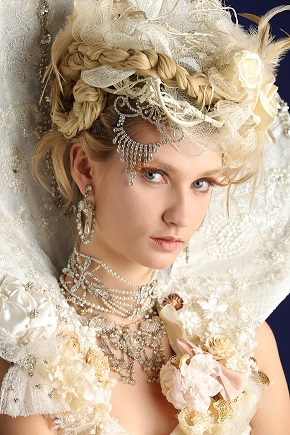
\includegraphics[width=3.5cm]{author.jpg}}},{}]
\end{window}

姓名:张 三

性别:男

出生年月:1985~年~00~月~00~日

民族:汉

籍贯:上海市

研究方向:图形图像处理

简历:

从这里开始写简历

200X.9-200X.7  XX大学XX专业个人简历,从大学起。

200X.9-200X.7  XX大学XX专业个人简历,从大学起。

200X.9-200X.7  XX大学XX专业个人简历,从大学起。

200X.9-200X.7  XX大学XX专业个人简历,从大学起。

200X.9-200X.7  XX大学XX专业个人简历,从大学起。

\cleardoublepage

%%----------  其他附录, 如不需要可用 % 注释掉下面几行
% !TEX TS-program = XeLaTeX
% !TEX encoding = UTF-8 Unicode

%%%%%%%%%%%%%%%%%%%%%%%%%%%%%%%%%%%%%%%%%%%%%%%%%%%%%%%%%%%%%%%%%%%%%%
%
%  哈尔滨工程大学学位论文 XeLaTeX 模版 —— 其他附加文件 app01.tex
%
%  版本:1.0.0
%  最后更新:
%  修改者:Leo LiWenhui lwh@hrbeu.edu.cn
%  修订者:
%  编译环境1:Ubuntu 12.04 + TeXLive 2013/2014
%  编译环境2:Windows 7/8  + TeXLive 2013/2014
%
%%%%%%%%%%%%%%%%%%%%%%%%%%%%%%%%%%%%%%%%%%%%%%%%%%%%%%%%%%%%%%%%%%%%%

\appendix{附录~A~~附录内容名称}

以下内容可放在附录之内:

\begin{asparaenum}
\item 正文内过于冗长的公式推导;
\item 方便他人阅读所需的辅助性数学工具或表格;
\item 重复性数据和图表;
\item 论文使用的主要符号的意义和单位;
\item 程序说明和程序全文。
\end{asparaenum}

这部分内容可省略。


\cleardoublepage
% !TEX TS-program = XeLaTeX
% !TEX encoding = UTF-8 Unicode

%%%%%%%%%%%%%%%%%%%%%%%%%%%%%%%%%%%%%%%%%%%%%%%%%%%%%%%%%%%%%%%%%%%%%%
%
%  哈尔滨工程大学学位论文 XeLaTeX 模版 —— 其他附加文件 app02.tex
%
%  版本:1.0.0
%  最后更新:
%  修改者:Leo LiWenhui lwh@hrbeu.edu.cn
%  修订者:
%  编译环境1:Ubuntu 12.04 + TeXLive 2013/2014
%  编译环境2:Windows 7/8  + TeXLive 2013/2014
%
%%%%%%%%%%%%%%%%%%%%%%%%%%%%%%%%%%%%%%%%%%%%%%%%%%%%%%%%%%%%%%%%%%%%%

\appendix{附录~B~~哈尔滨工程大学学位论文撰写规范}

 \hei 说明:
 \kai
 这些规定偶有变动。

 请仔细查阅当年拿到的《哈尔滨工程大学研究生学位论文规范》。

 若发现不一致的地方, 请与我联系(lwh@vip.163.com)。

\vspace*{0.5cm}

\song
学位论文是表明作者从事科学研究取得创造性结果或有了新的见解,并以此为内容撰写而成的学术论文。研究生学位论文展示了研究生在科学研究工作中取得的成果并全面反映了研究生对本学科基础理论和专门知识的掌握程度,是申请和授予相应学位的基本依据。学位论文撰写是研究生培养过程的基本训练之一,必须按照确定的规范认真执行。

本论文规范按照《科学技术报告、学位论文和学术论文的编写格式》(GB 7713-87)、《文后参考文献著录规则》(GB 7714-87)以及《标准化工作导则标准编写的基本规定》(GB/T1.1-1993)制定。

本论文规范适用于我校博士、硕士研究生和本科生。学位论文除在字数、理论研究的深度及创造性成果等方面的要求不同以及特殊说明外,对其撰写规范的要求基本一致。


{\hei 一、论文装订格式的排列顺序\footnote{硕士研究生和本科生的要求与博士生有不同。}}

(一)封面

(二)论文英文题目

(三)原创性及授权声明

(四)学位论文使用授权书

(五)博士生自认为的论文创新点

(六)目录

(七)中文摘要

(八)英文摘要

(九)引言

(十)正文

(十一)中外文参考文献

(十二)攻博期间发表的与学位论文相关的科研成果目录

(十三)后记/致谢

{\hei 二、论文印制规格及要求}

(一)论文用A4张(210×297mm)标准大小的白纸打印;

(二)\colorbox{yellow}{正文部分研究生论文要求双面印制,本科生论文单面印制};

(三)版心尺寸160×241mm,版心页边距上、下设置为28mm,左、右设置为25mm,页眉、页脚设置为20mm。装订时上、下、右各切除3mm,学位论文成品版面大小为207mm*291mm。

{\hei 三、论文封面格式}

(一)分类号:必须在封面左上角注明分类号,一般应注明《中国图书资料分类法》的类号,
同时尽可能注明《国际十进分类法UDC》的类号.

(二)密级:论文必须按国家规定的保密条例在右上角注明密级(如系公开型论文则可不注明密级)。

(三)论文题目:题目必须用楷体标准一号字标注于明显的位置,应是集中概括论文最重要的内容,
一般不超过20个字,以有助于选定关键词和编制题录。题目不能用缩略词,首字母缩写字、字符、
代号和公式等,题目语意未尽,可用副标题补充说明。外语专业的论文题目一般采用英文,英文题目不宜超过10个实词。

(四)论文作者姓名:

(五)论文指导教师姓名:指导教师姓名必须是填写当年被学校批准招收博士生的教师。

(六)专业名称:专业名称必须是我校已有学位授予权的学科专业,并按国家颁布的学科专业目录中一级学科或二级学科名称印制。

(七)书脊(专指博士学位论文):书脊上应用仿宋体四号字于上方标明论文题目,下方注明研究生姓名。

(八)论文封面:统一用120克铜版纸,封面底色为白色。

{\hei 四、论文英文题目}

论文英文题目专用一页纸,“英文题目”用宋体二号字,其下“研究生姓名”用宋体四号字;外语专业应为中文题目。

{\hei 五、原创性及授权声明}

“原创性及授权声明”用黑体小二号字,内容用宋体四号字。

为了加强学风、学术道德建设,规范学术行为,提高学位论文质量,确保学位授予的权威性、严肃性,学校对学位论文撰写特别强调以下几点:

(一)凡申请学位人员须对自己的学位论文负责,在提交的学位论文的英文题目后页(中文摘要前页)增设一页书面声明,即“郑重声明”。

(二)学位论文中的引证、引述处须注明出处。

(三)学位论文后所附参考文献,必须是申请学位人员真正阅读和参考过的文献。

(四)合作科研及成果,应在致谢或后记中有相关说明,避免产权纠纷。

(五)学位论文中没有原创性及授权声明的,不能参加论文答辩。

{\hei 六、中文摘要}

“中文摘要”用黑体小二号字,内容用宋体小四号字,页码用罗马数字单独编排,并标注在每页页脚中部。

{\hei 七、英文摘要}

“英文摘要”用加粗Times New Roman小二号字,内容用Times New Roman小四号字,页码续接中文摘要的页码。

{\hei 八、论文关键词}

每篇论文必须选取3--5个以上中、英文关键词,排在其论文摘要的左下方,用黑体小四号字。

{\hei 九、目录}

目录是论文的提纲,也是论文组成部分的小标题.
排列顺序是:1、中文摘要 2、英文摘要 3、引言 4、正文章节 5、中外文参考文献 6、攻博期间发表的科研成果目录
7、后记(可不要此项)。 并对每项标明页码。

{\hei 十、引言(绪论)}

论文的页码由引言(绪论)的首页开始,作为第1页,并为右页,一律用阿拉伯数字连续编排页码,必须统一标注在每页页脚中部。

{\hei 十一、正文}

正文是学位论文的核心部分,必须由另页开始,一级标题之间换页,二级标题之间空行;内容一律用宋体小四号字,
字间距设置为标准字间距,行间距设置为最小值20磅,各章、节应有序号。

{\hei 十二、参考文献}

参考文献用黑体四号字,内容用宋体五号字。

{\hei 十三、学位论文印刷份数}

由培养单位根据需要决定印刷份数. 在学位论文定稿后,可先印刷数份给论文评阅人和答辩委员,
然后根据论文评阅人和答辩委员对论文的意见进行修改后,才能正式印刷,提交学校存档。

{\hei 十四、论文制作时不须页眉}

\cleardoublepage

%%%%%%%%%%%% 到这就结束了! %%%%%%%%%%%%%%%%%%%%%%%%%%%%
\end{document}
